%%%%%%%%%%%%%%%%%%%%%%%%%%%%%%%%%%%%%%%%%%%%%%%%%%%%%%%
%% Bachelor's & Master's Thesis Template             %%
%% Copyleft by Artur M. Brodzki & Piotr Woźniak      %%
%% Faculty of Electronics and Information Technology %%
%% Warsaw University of Technology, 2019-2020        %%
%%%%%%%%%%%%%%%%%%%%%%%%%%%%%%%%%%%%%%%%%%%%%%%%%%%%%%%

\documentclass[
    left=2.5cm,         % Sadly, generic margin parameter
    right=2.5cm,        % doesnt't work, as it is
    top=2.5cm,          % superseded by more specific
    bottom=3cm,         % left...bottom parameters.
    bindingoffset=6mm,  % Optional binding offset.
    nohyphenation=false % You may turn off hyphenation, if don't like.
]{eiti/eiti-thesis}

\langpol % Dla języka angielskiego mamy \langeng
\graphicspath{{img/}}             % Katalog z obrazkami.
\addbibresource{bibliografia.bib} % Plik .bib z bibliografią

% \usepackage[T1]{fontenc}
% \usepackage[scaled]{beramono}

\usepackage{color}
\definecolor{bluekeywords}{rgb}{0.13,0.13,1}
\definecolor{greencomments}{rgb}{0,0.5,0}
\definecolor{redstrings}{rgb}{0.9,0,0}

\usepackage[utf8]{inputenc}
\usepackage{listings}

\lstset{literate={↑}{$\uparrow$}1 {↓}{$\downarrow$}1 {←}{$\leftarrow$}1 {→}{$\rightarrow$}1}


\lstset{language=[Sharp]C,
showspaces=false,
showtabs=false,
breaklines=true,
showstringspaces=false,
breakatwhitespace=true,
escapeinside={(*@}{@*)},
commentstyle=\color{greencomments},
keywordstyle=\color{bluekeywords}\bfseries,
stringstyle=\color{redstrings},
breaklines=true
}

\lstdefinelanguage{JavaScript}{
  keywords={break, case, catch, continue, debugger, default, delete, do, else, finally, for, function, if, in, instanceof, new, return, switch, this, throw, try, typeof, var, void, while, with},
  morecomment=[l]{//},
  morecomment=[s]{/*}{*/},
  morestring=[b]',
  morestring=[b]",
  sensitive=true,
  breaklines=true
}

\newcommand{\tocless}[2]{\bgroup\let\addcontentsline=\nocontentsline#1{#2}\egroup}

\begin{document}

%--------------------------------------
% Strona tytułowa
%--------------------------------------
\MasterThesis % Dla pracy inżynierskiej mamy \EngineerThesis
\instytut{Automatyki i Informatyki Stosowanej}
\kierunek{Informatyka}
\specjalnosc{Systemy Internetowe Wspomagania Zarządzania}
\title{
    Implementacja gry strategicznej Statki, opracowanie algorytmów decyzyjnych oraz analiza ich skuteczności.
}
\engtitle{ % Tytuł po angielsku do angielskiego streszczenia
    Implementation of a Battleships strategy game, development of decision making algorithms and an analysis of their effectiveness.
}
\author{Jakub Kalinowski}
\album{284234}
\promotor{dr Sebastian Plamowski}
\date{\the\year}
\maketitle

%--------------------------------------
% Streszczenie po polsku
%--------------------------------------
\cleardoublepage % Zaczynamy od nieparzystej strony
\streszczenie{
Celem niniejszej pracy było zaimplementowanie gry strategicznej Statki i opracowanie algorytmów decyzyjnych, aby ostatecznie przeanalizować skuteczność poszczególnych algorytmów. Według wstępnych założeń, algorytmy miały opierać się na heurystykach. Analiza skuteczności miała opierać się na bezpośrednich starciach różnych algorytmów oraz na starciach człowiek - algorytm.
\\ \indent W pracy omówione zostały zagadnienia związane z heurystykami, z punktu widzenia logiki oraz informatyki. Opisane zostały typowe zastosowania heurystyk.
\\ \indent W dalszej części pracy opisane zostało zaimplementowane rozwiązanie - wykorzystany stack technologiczny, logika aplikacji, implementacja poszczególnych heurystyk. Opisane zostało działanie najważniejszych fragmentów kodu.
\\ \indent Kolejnym krokiem było testowanie algorytmów. W tym celu napisane zostały testy jednostkowe, które zestawiały przeciwko sobie poszczególne heurystyki. Na podstawie wyników tych starć dokonano analizy porównawczej. Podjęto również próbę analizy starć pomiędzy algorytmami oraz ludźmi.
\\ \indent W ostatniej części pracy podsumowane zostały wyniki oraz opisane zostały wnioski - co można było zrobić lepiej, jakie są możliwości rozwoju aplikacji.
}
\slowakluczowe heurystyki, statki, algorytmy, vue.js, .net

%--------------------------------------
% Streszczenie po angielsku
%--------------------------------------
\newpage
\abstract {
The purpose of this study was to implement the strategy game Battleships and to develop decision-making algorithms to analyze the effectiveness of the various algorithms. According to the initial assumptions, the algorithms were to be based on heuristics. The effectiveness analysis was to be based on direct clashes between different algorithms and on human-algorithm clashes.
\\ \indent The paper discusses issues related to heuristics, from the point of view of logic and computer science. Typical applications of heuristics are described.
\\ \indent The following part of the work describes the implemented solution - the technology stack used, the application logic, the implementation of individual heuristics. The most important code fragments were highlighted and described.
\\ \indent The next step was to test the algorithms. For this purpose, unit tests were written that pitted individual heuristics against each other. Based on the results of these clashes, a comparative analysis was made.  An attempt was also made to analyze clashes between the algorithms and players.
\\ \indent In the last part of the work the results were summarized, and conclusions were written - what could have been done better, what are the possibilities for the development of the application.
}
\keywords heuristics, battleships, algorithms, vue.js, .net

%--------------------------------------
% Oświadczenie o autorstwie
%--------------------------------------
\cleardoublepage  % Zaczynamy od nieparzystej strony
\pagestyle{plain}
\makeauthorship

%--------------------------------------
% Spis treści
%--------------------------------------
\cleardoublepage % Zaczynamy od nieparzystej strony
\tableofcontents

%--------------------------------------
% Rozdziały
%--------------------------------------
\cleardoublepage % Zaczynamy od nieparzystej strony
\pagestyle{headings}

\newpage % Rozdziały zaczynamy od nowej strony.
\section{Wstęp}

\subsection{Wprowadzenie}
\indent\ Heurystyki, czyli uproszczone metody podejmowania decyzji, pomagają nam w codziennym życiu przy  podejmowaniu różnych decyzji, nawet jeśli nie jesteśmy tego do końca świadomi. Często korzystamy z heurystyk, aby szybciej podjąć decyzję - nie mamy wtedy jednak pewności że będzie to decyzja optymalna. "Heurystyka dostępności" jest często stosowana do szacowania prawdopodobieństwa zdarzeń, na podstawie tego jak łatwo jest nam przywołać przykłady wystąpienia tego zdarzenia - na przykład jeśli wielokrotnie słyszymy że na zaparkowany samochód spadło drzewo, będziemy unikać parkowania pod drzewem \cite{tversky74}.
\\ \indent Heurystyki w kontekście informatyki również ułatwiają rozwiązywanie problemów, których złożoność obliczeniowa jest na tyle duża, że ma to bardzo negatywny wpływ na czas wykonywania obliczeń. Jako przykład może służyć problem komiwojażera - dla podanych miast oraz dystansów między nimi, musimy wyznaczyć najkrótszą drogę wiodącą z miasta A do B, która przechodzi przez wszystkie inne miasta. Dla małej liczby miast, problem można rozwiązać metodą brute-force, obliczając wszystkie możliwe ścieżki i wybierając najkrótszą. Jednak z każdym dodanym do zadania miastem, znacznie wzrasta liczba możliwych ścieżek - a wraz z nią czas potrzebny na obliczenia. W tym celu Job Bentley zaproponował uproszczony algorytm, który nie bierze pod uwagę wszystkich ścieżek. Zamiast tego, dla każdego kolejnego kroku, wybiera po prostu najbliższe miasto. Ostatecznie wybrana ścieżka nie zawsze będzie faktycznie tą możliwie najkrótszą, ale będzie do niej zbliżona \cite{Hjeij2023}
\\ \indent Niniejsza praca zagłębia się w zastosowanie heurystyk w informatyce, a konkretnie w grach komputerowych. Jest do świetne narzędzie do implementacji algorytmów decyzyjnych, z których korzystają komputerowi przeciwnicy w grze. Szczególnie we wpółczesnych grach z otwartym światem, podejmowanie decyzji przez przeciwników nie może za bardzo obciążać zasobów procesora, ponieważ są one również potrzebne do obliczeń fizyki gry, symulacji otaczającego gracza świata, logiki gry, etc.
\\ \indent 

\subsection{Cel pracy}
\indent Celem niniejszej pracy była implementacja turowej gry strategicznej Statki oraz analiza skuteczności algorytmów decyzyjnych przeciwnika. W implementacji istotne było zapewnienie możliwości archiwizacji zakończonych rozgrywek w bazie danych, aby później możliwa była ich analiza.

\subsection{Metodologia}
\indent Przedmiotem badania była ocena skuteczności zaimplementowanych algorytmów. Na koniec pracy powinniśmy znać odpowiedzi na pytania:
\begin{enumerate}
  \item Który algorytm decyzyjny jest najbardziej skuteczny?
  \item Co ma wpływ na skuteczność algorytmów?
  \item Czy skuteczność algorytmów różni się w zależności od tego czy gra przeciwko człowiekowi, czy innemu algorytmowi?
\end{enumerate}
Aby opowiedzieć na te pytania, przeprowadzimy analizę statystyczną rozgrywek zapisanych w bazie danych.         % Wygodnie jest trzymać każdy rozdział w osobnym pliku.
\newpage % Rozdziały zaczynamy od nowej strony.
\section{Gra strategiczna Statki – podstawowe zasady i historia}

\subsection{Historia gry}
\indent\ Gra Statki, znana również jako "Battleships", to popularna gra strategiczna, której korzenie sięgają początku XX wieku. Jest to gra turowa dla dwóch graczy, którzy starają się zatopić flotę przeciwnika oddając na zmianę strzały na planszę przeciwnika. Gracze nie widzą planszy przeciwnika, po każdym oddanym strzale dostają jedynie informację zwrotną, czy trafili w statek.
\\ \indent Pierwsze wersje gry "Statki" to gry papierowe, które były popularne wśród żołnierzy w trakcie I Wojny Światowej. Do gry potrzebne były jedynie 2 kartki oraz ołówek, więc można było w nią grać właściwie wszędzie. \cite{historyWiki}
\\ \indent Od lat 30 XX wieku, dostępne były komercyjne wersje gry - gracze mogli kupić gotowe papierowe plansze do gry, aby własnoręcznie ich nie rysować. W 1967 roku firma Milton Bradley zaczęła produkować prawdopodobnie najbardziej znaną wersję gry, składającą się z plastikowych planszy oraz statków \cite{historyWiki} \cite{museumOfGames}.

\begin{figure}[!h]
    \label{fig:milton-bradley-game}
    \centering 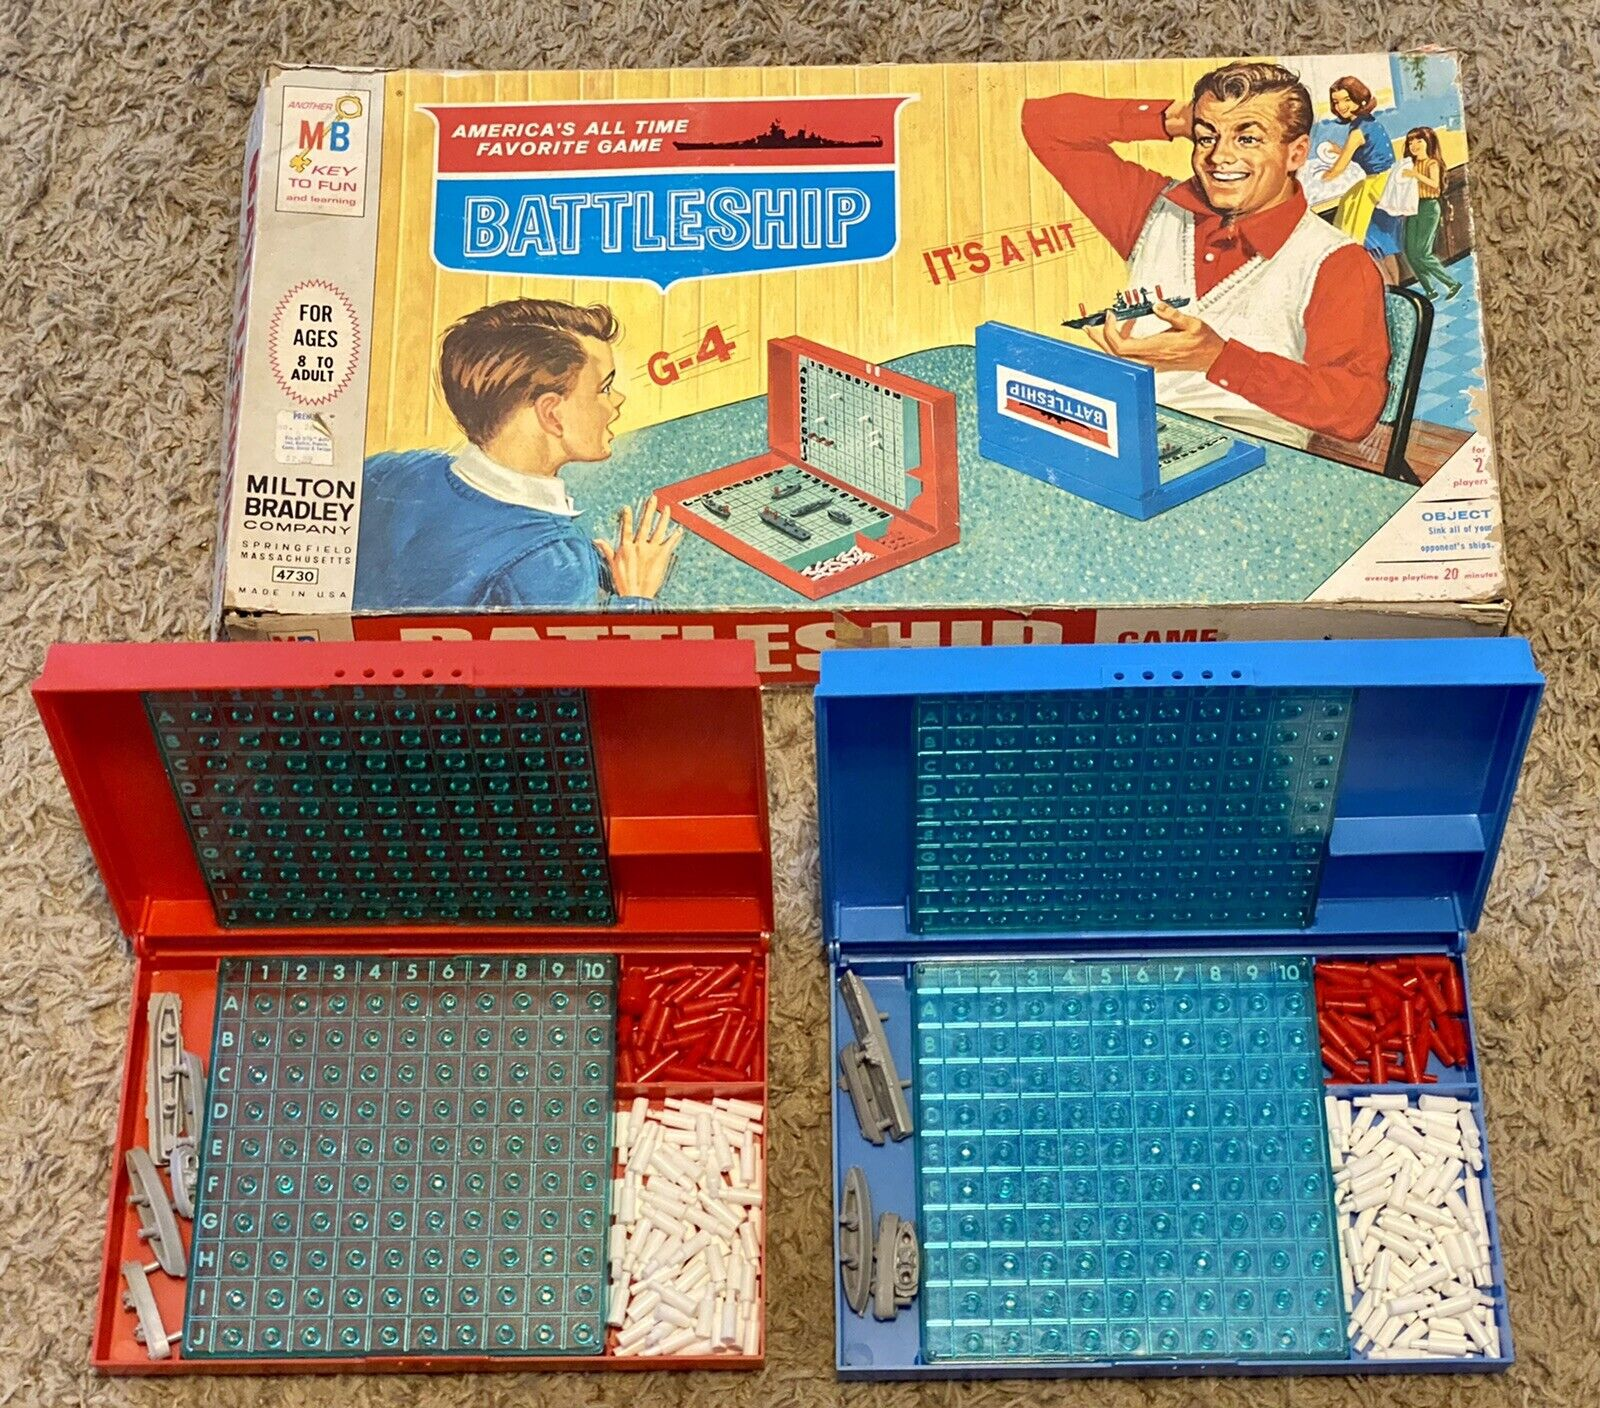
\includegraphics[width=0.8\linewidth]{img/milton_bradley_game.jpg}
    \caption{Gra Battleship wyprodukowana przez firmę Milton Bradley \cite{eBay}.}
\end{figure}

 \indent Z biegiem lat, gra Statki ewoluowała, przyjmując różne formy. W latach 70. XX wieku pojawiła się pierwsza wersja elektroniczna gry, dostępna na komputerach Z80 Compucolor, napisana w języku BASIC. Wraz z rozwojem PC, zaczęło pojawiać się coraz więcej wersji gry \cite{historyWiki} \cite{museumOfGames}.

 \begin{figure}[!h]
    \label{fig:commodore_64}
    \centering 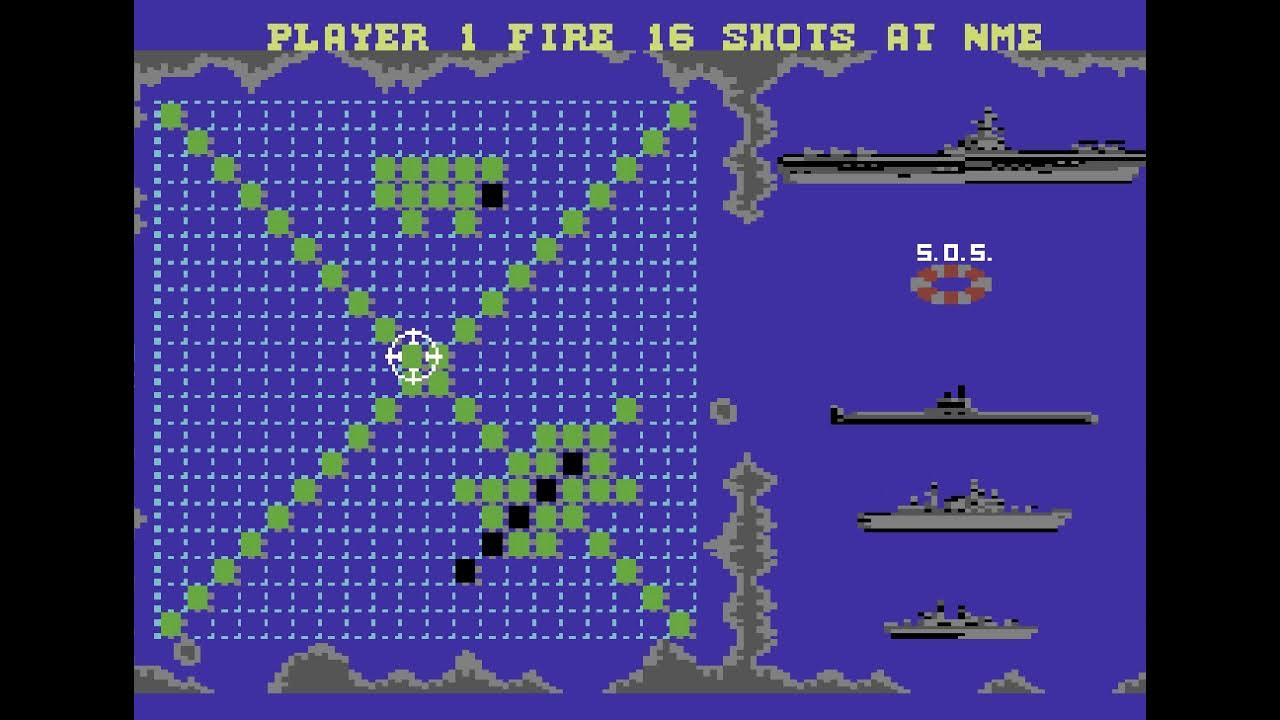
\includegraphics[width=0.8\linewidth]{img/commodore_64.jpg}
    \caption{Ujęcie z gry \emph{Battleship} dostępnej na komputerze Commodore 64 \cite{commodore64}.}
\end{figure}

\indent Gra Statki jest znanym elementem kultury popularnej na całym świecie, na jej podstawie w 2012 roku powstał nawet film "Battleship".
\subsection{Zasady}
\indent\ Zasady gry Statki różnią się w zależności od wersji. Zasady przyjęte w niniejszej pracy:
\begin{itemize}
  \item Gracze mają do dyspozycji po jednym statku o danej długości, zaczynając od jednomasztowca, kończąc na pięciomasztowcu.
  \item Dany statek musi znajdować się w linii prostej (nie może na przykład być "złamany" i tworzyć literę L).
  \item Plansza ma wymiary 10 na 10 komórek.
  \item Gracz może wybrać czy statki mogą się ze sobą stykać bokami lub wierzchołkami. Ma to na celu dodanie dodatkowej zmiennej do analizy skuteczności algorytmów.
\end{itemize}

Różnorodność zasad to być może coś, co przyczyniło się do popularności tej gry - gracze mogą zmieniać zasady, tak aby rozgrywka była dla nich jak najciekawsza. Gra ograniczona wieloma zasadami, takimi jak to, że statki nie mogą ze sobą sąsiadować, prowadzi do bardziej analitycznej rozgrywki - gracze mogą eliminować z rozważań pola, na których zgodnie z zasadami nie mogą znajdować się statki. Gdy nie ma zasad ograniczających rozstawienie statków, gra staje się dużo bardziej losowa.    % Umożliwia to również łatwą migrację do nowej wersji szablonu:
\newpage % Rozdziały zaczynamy od nowej strony.
\section{Algorytmy}
\subsection{Wprowadzenie do algorytmów}

Algorytmy stanowią podstawę działania każdego programu komputerowego. Są to zestawy kroków, które prowadzą do rozwiązania określonego problemu. Każdy algorytm można opisać za pomocą języka formalnego, który jest zrozumiały dla komputera. W kontekście informatyki, algorytmy nie tylko rozwiązują problemy, ale także optymalizują procesy obliczeniowe, minimalizując czas i zasoby potrzebne do uzyskania wyniku\cite{algorithms}.

\subsection{Klasyfikacja algorytmów}

Algorytmy można klasyfikować według różnych kryteriów, w zależności od ich struktury, sposobu działania, oraz rodzaju problemów, które rozwiązują. Oto kilka głównych kategorii:

\begin{itemize}
    \item{\textbf{Algorytmy deterministyczne i niedeterministyczne}}
    
    Algorytmy deterministyczne zawsze prowadzą do tego samego wyniku, jeśli zostaną uruchomione z tymi samymi danymi wejściowymi. Przykładem jest algorytm sortowania bąbelkowego (bubble sort) [2]. Z kolei algorytmy niedeterministyczne mogą dawać różne wyniki przy tych samych danych wejściowych, jak np. algorytmy genetyczne \cite{cohen1979non}.
    
    \item{\textbf{Algorytmy dokładne i przybliżone}}
    
    Algorytmy dokładne znajdują optymalne rozwiązanie problemu, jednak często wymagają dużych zasobów obliczeniowych. Przykładem jest algorytm znajdowania najkrótszej ścieżki w grafie (algorytm Dijkstry). Algorytmy przybliżone, jak heurystyki, oferują rozwiązanie, które może nie być optymalne, ale jest uzyskane znacznie szybciej \cite{trevisan}.
    
    \item{\textbf{Algorytmy iteracyjne i rekurencyjne}}

    Algorytmy iteracyjne rozwiązują problem poprzez powtarzanie określonych operacji, aż do osiągnięcia pożądanego rezultatu. Algorytmy rekurencyjne natomiast rozwiązują problem, wywołując samą siebie na mniejszych podproblemach. Przykładem algorytmu rekurencyjnego jest algorytm wyszukiwania binarnego \cite{recursiveVsIterative}.
    
\end{itemize}

\subsection{Przykłady popularnych algorytmów}
\begin{itemize}
    \item{\textbf{Algorytmy sortowania}}

    Sortowanie to proces porządkowania elementów w określonej kolejności. Istnieje wiele algorytmów sortowania, takich jak quicksort, mergesort, czy bubble sort. Każdy z nich ma swoje wady i zalety w zależności od danych wejściowych i kontekstu, w którym jest stosowany \cite{algorithms}.
    
    \item{\textbf{Algorytmy wyszukiwania}}

    Algorytmy wyszukiwania służą do znalezienia określonego elementu w strukturze danych. Przykładami są algorytm wyszukiwania liniowego oraz algorytm wyszukiwania binarnego, który działa znacznie szybciej w posortowanych zbiorach danych \cite{sedgewick}.
    
    \item{\textbf{Algorytmy grafowe}}

    Algorytmy działające na grafach są kluczowe w wielu dziedzinach, od analizy sieci po optymalizację tras. Do najważniejszych należą algorytm Dijkstry do znajdowania najkrótszej ścieżki, algorytm Kruskala i algorytm Prima do znajdowania minimalnego drzewa rozpinającego \cite{algorithms}.
    
    \item{\textbf{Algorytmy sztucznej inteligencji}}

    Wraz z rozwojem sztucznej inteligencji, algorytmy AI zyskały na znaczeniu. Algorytmy te, takie jak algorytmy genetyczne, sieci neuronowe czy algorytmy uczące się, umożliwiają komputerom naśladowanie procesów myślowych człowieka, podejmowanie decyzji oraz uczenie się na podstawie danych \cite{Mitchell1996AnIT}.
    
\end{itemize}

\subsection{Złożoność obliczeniowa algorytmów}

Złożoność obliczeniowa odnosi się do ilości zasobów, takich jak czas i pamięć, które są potrzebne do wykonania algorytmu. Jest to kluczowy aspekt przy ocenie efektywności algorytmu. Złożoność obliczeniową wyraża się zazwyczaj w notacji O (Big O), która opisuje asymptotyczne zachowanie algorytmu, czyli jak rośnie jego czas wykonywania wraz ze wzrostem wielkości danych wejściowych \cite{artoOfProgramming}.

Przykłady:
\begin{itemize}
    \item{\textbf{O(1)}}

    Stała złożoność czasowa, niezależna od wielkości danych wejściowych.
    
    \item{\textbf{O(n)}}

    Złożoność liniowa, czas wykonywania rośnie proporcjonalnie do wielkości danych wejściowych.
    
    \item{\textbf{O(n^{2})}}

    Złożoność kwadratowa, czas wykonywania rośnie kwadratowo wraz ze wzrostem danych wejściowych.
    
\end{itemize}

\subsection{Znaczenie algorytmów w informatyce} Współczesna informatyka nie mogłaby istnieć bez algorytmów. Stanowią one fundament każdej aplikacji, od prostych programów po zaawansowane systemy komercyjne. Znajomość algorytmów i umiejętność ich optymalizacji jest kluczowa dla programistów, inżynierów oprogramowania oraz naukowców zajmujących się sztuczną inteligencją, big data czy analizą danych.
\newpage % Rozdziały zaczynamy od nowej strony.
\section{Heurystyki}

\subsection{Definicja i rola heurystyk}
\indent\ Termin "heurystyka" pochodzi od greckiego \emph{heurískō}, co oznacza \emph{znajdować/odkrywać} \cite{heuristicEtymology}. Heurystyki to uproszczone metody podejmowania decyzji, które umożliwiają szybkie i efektywne rozwiązywanie problemów.

Badania nad heurystykami zostały rozpoczęte przez psychologów Amosa Tversky'ego oraz Daniela Kahnemana w latach 70 XX wieku. Opisane przez nich heurystyki stanowiły wytłumaczenie dla systematycznych odstępstw od teoretycznie bardziej racjonalnych decyzji. Podczas podejmowania decyzji ludzie stosują skróty myślowe, które ułatwiają im podjęcie decyzji, ale jednocześnie sprawiają, że są bardziej podatni na błędy poznawcze (ang. cognitive bias). Tversky i Kahneman sformułowali wiele heurystyk używanych w psychologii do dziś, między innymi heurystyki dostępności, zakotwiczenia i dostosowania czy reprezentatywności \cite{tversky74} \cite{psychol} \cite{laibson}.

Przykłady heurystyk:
\begin{itemize}
    \item{\textbf{Dostępności}}: Oceniamy prawdopodobieństwo zdarzenia, na podstawie tego jak łatwo możemy przywołać odpowiednie przykłady. Jeśli jakieś zdarzenie lub informacja jest bardziej dostępna w naszej pamięci, mamy tendencję do przeceniania jej prawdopodobieństwa wystąpienia \cite{tversky74}.
    \item{\textbf{Zakotwiczenia i dostosowania}}: Przy podejmowaniu decyzji polegamy na początkowej informacji (zakotwiczeniu), ale nie dostosowujemy wagi tej informacji po otrzymaniu nowych danych. Przykładem może być sytuacja, gdy konsument początkowo widzi wysoką cenę produktu. Jeśli następnie zobaczy obniżkę, pomyśli że jest to bardzo korzystna oferta. W przeciwnej sytuacji, jeśli najpierw zobaczy przeceniony produkt, a następnie w normalnym wariancie cenowym, będzie wydawał mu się zbyt drogi \cite{tversky74, pricing}.
    \item{\textbf{Reprezentatywności}}: Na podstawie stereotypu, oceniamy prawdopodobieństwo przynależności osoby do danej grupy. Przykładowo: jeśli widzimy zgarbionego, bladego chłopaka w okularach i zostaniemy zapytani czy bardziej prawdopodobne jest to czy jest informatykiem czy rolnikiem, wybierzemy pierwszą opcję. Z logicznego punktu widzenia nie jest to dobry wybór, ponieważ na świecie jest więcej rolników niż informatyków. Dzieje się tak, ponieważ wymienione cechy pasują do istniejącego w naszej głowie stereotypu \cite{tversky74} \cite{sudeep}.
\end{itemize}

\subsection{Heurystyki w grach strategicznych}
W kontekście gier strategicznych, heurystyki są kluczowe dla efektywnego zarządzania zasobami, planowania i adaptacji strategii. Komputerowi przeciwnicy korzystają z heurystyk, aby naśladować ludzkie myślenie i podejmowanie decyzji, co czyni rozgrywkę bardziej wymagającą i interesującą dla graczy.

Przykładowe heurystyki wykorzystywane w grach:
\begin{itemize}
  \item \textbf{Heurystyki oparte na odległości:} Przykładem jest heurystyka najkrótszej ścieżki, która służy do oceny odległości między jednostkami lub celami w grze, co pomaga w planowaniu ruchów i ataków \cite{inproceedings}.
  \item \textbf{Heurystyki oparte na priorytetach:} Pozwalają graczom ustalać priorytety dla różnych celów lub działań. Na przykład, w grach RTS (Real-Time Strategy), przeciwnik może priorytetowo traktować budowanie zasobów lub atakowanie gracza w początkowej fazie gry \cite{Ontan2013ASO}.
  \item \textbf{Heurystyki oparte na doświadczeniu:} Korzystają z wcześniej zdobytych doświadczeń lub wyników gier do podejmowania decyzji. Przykładem może być rozpoznawanie wzorców w ruchach gracza i dostosowywanie strategii na ich podstawie \cite{Weber_Mateas_Jhala_2011}.
\end{itemize}

\subsection{Heurystyki zastosowane w pracy}
\begin{enumerate}
  \item \textbf{Heurystyka maksymalizacji zysku ze strzału}
  
   Przeciwnik analizuje ile istnieje możliwości ustawienia statków dla danej komórki. Na rysunku 3.1 widoczna jest mapa prawdopodobieństwa, obliczona na podstawie tej heurystyki. Wartości widoczne na każdej komórce oznaczają na ile sposobów można ustawić dostępne statki na danej komórce. Pola będące krawędziami planszy mają wartość 10, ponieważ może na nich znaleźć się każdy ze statków w pionie i w poziomie, w obu przypadkach w dokładnie jednej pozycji. Pola znajduujące się bliżej środka mapy mają większe wartości, ponieważ statki mogą znajdować się na nich w wielu pozycjach. Na przykład poziomy trzymasztowiec może znajdować się na polu X, Y na 3 sposoby. Poniżej wymienione są jego możliwe współrzędne:
  \begin{itemize}
      \item (X-2,Y), (X-1,Y), (X,Y)
      \item (X-1,Y), (X,Y), (X+1,Y)
      \item (X,Y), (X+1,Y), (X+2,Y)
  \end{itemize}

  Heurystyka maksymalizacji zysku ze strzału pozwala na wykonywanie jak najbardziej efektywnych strzałów pod kątem eliminacji możliwych rozstawień statków.
  
  
  \begin{figure}[!h]
    \label{fig:mapa-prawdopodobienstwa-heurystyka-max-zysku}
    \centering 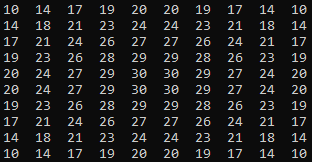
\includegraphics[width=0.5\linewidth]{img/probabilityMapStart.PNG}
    \caption{Mapa prawdopodobieństwa podczas rozpoczęcia gry, przy wykorzystaniu heurystyki maksymalizacji zysku ze strzału.}
\end{figure}
  
  \item \textbf{Heurystyka najbardziej prawdopodobnej lokalizacji na podstawie trafień}

  
  Przeciwnik analizuje swoje dotychczasowe trafienia i skupia się na ostrzale komórek sąsiadujących z pojedynczymi trafieniami oraz wzdłuż linii kilku sąsiadujących trafień. Zatopione statki nie są brane pod uwagę. Jeśli żaden statek nie został jeszcze trafiony, strzały oddawane są losowo. Na rysunku 3.2 widoczne są dwie mapy prawdopodobieństwa. Piersza mapa przedstawia sytuację, gdzie trafiona została pojedyncza komórka - wtedy wszystkie sąsiadujące komórki mogą zawierać pozostałą część statku. Na drugim rysunku trafione zostały dwie sąsiadujące komórki - wtedy rozważane są jedynie komórki sąsiadujące, będące na przedłużeniu linii dotychczasowych trafień. Wartości przedstawione na mapie prawdopodobieństwa są umówne - 50 dla komórek sąsiadujących z pojedynczym trafieniem oraz 100 dla komórek sąsiadujących z serią trafień.
  \begin{figure}[!h]
    \label{fig:mapa-prawdopodobienstwa-heurystyka-trafien}
    \centering 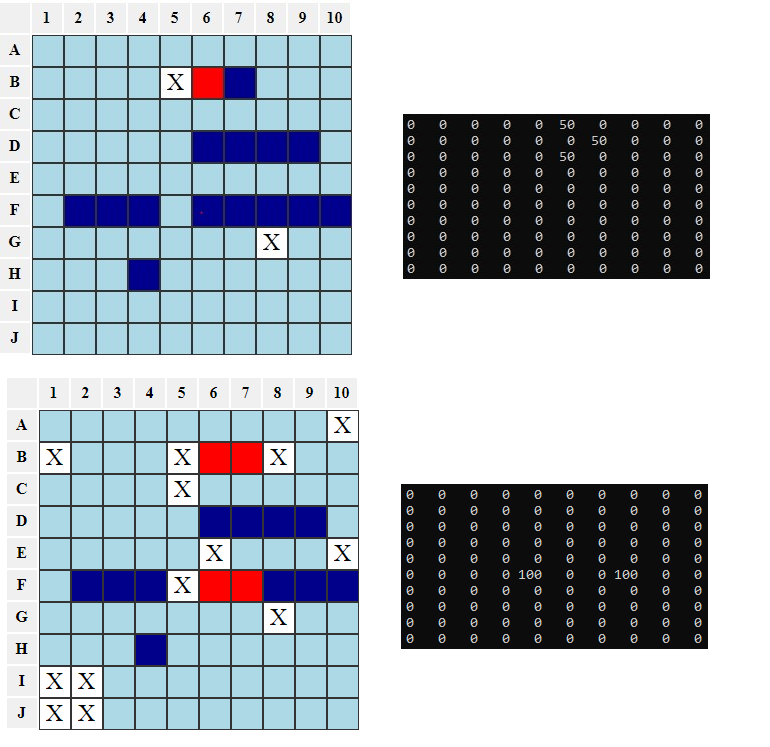
\includegraphics[width=0.9\linewidth]{img/hit-heuristic.png}
    \caption{Mapy prawdopodobieństwa dla dwóch stanów planszy gracza, przy wykorzystaniu heurystyki najbardziej prawdopodobnej lokalizacji na podstawie trafień.}
\end{figure}
  
  \item \textbf{Heurystyka maksymalizacji zysku priorytetyzująca dłuższe statki}
  
  Bardzo podobna do już wspomnianej heurystyki maksymalizacji zysku, z jedną różnicą - priorytetyzowane są dłuższe statki. W podstawowej wersji heurystyki, jeśli statek mógł znajdować się na komórce (X,Y) w liczbie Z pozycji, dodawaliśmy Z do tej komórki na mapie prawdopodobieństwa. Teraz dodajemy
  \begin{align*}
    Z * L^2
\end{align*}
Gdzie L to długość statku.
  \\ Heurystyka ta pozwala na szybszą eliminację dużych statków.
    \begin{figure}[!h]
    \label{fig:mapa-prawdopodobienstwa-max-zysku-wazona}
    \centering 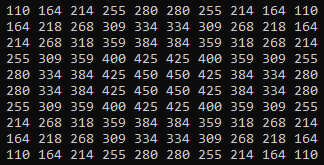
\includegraphics[width=0.5\linewidth]{img/max-benefit-weighted.PNG}
    \caption{Mapa prawdopodobieństwa podczas rozpoczęcia gry, przy wykorzystaniu heurystyki maksymalizacji zysku priorytetyzującej dłuższe statki.}
    \end{figure}

  \item \textbf{Heurystyka maksymalizacji zysku oraz najbardziej prawdopodobnej lokalizacji na podstawie trafień}
  
  Połączenie heurystyki maksymalizacji zysku ze strzału (1) oraz heurystyki najbardziej prawdopodobnej lokalizacji na podstawie trafień (2). Ulepszenie podstawowej heurystyki najbardziej prawdopodobnej lokalizacji na podstawie trafień - zamiast losowo ostrzeliwać pola, gdy żadne nie jest jeszcze trafione, teraz strzały oddawane są w pola, które wskazuje heurystyka maksymalizacji zysku. Wagi obu heurystyk są tak dopasowane, aby heurystyka dotychczasowych trafień miała większy wpływ na wybór komórki do ostrzału.

    \begin{figure}[!h]
    \label{fig:mapa-prawdopodobienstwa-heurystyka-laczona}
    \centering 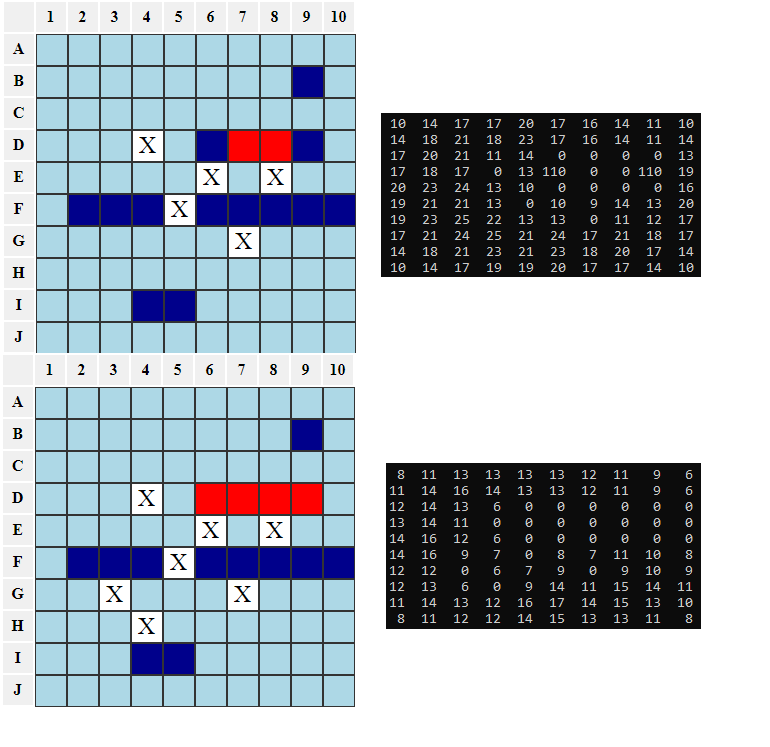
\includegraphics[width=0.9\linewidth]{img/complete-heuristic.png}
    \caption{Mapa prawdopodobieństwa podczas rozpoczęcia gry, przy wykorzystaniu heurystyki maksymalizacji zysku oraz najbardziej prawdopodobnej lokalizacji na podstawie trafień.}
    \end{figure}

  \item \textbf{Heurystyka maksymalizacji zysku oraz najbardziej prawdopodobnej lokalizacji na podstawie trafień priorytetyzująca dłuższe statki}
  
  Połączenie heurystyki maksymalizacji zysku ze strzału priorytetyzującej dłuższe statki (3) oraz heurystyki najbardziej prawdopodobnej lokalizacji na podstawie trafień (2). Wagi obu heurystyk są tak dopasowane, aby heurystyka dotychczasowych trafień miała większy wpływ na wybór komórki do ostrzału. W sytuacji, gdy żadne pole nie jest jeszcze trafione, priorytetyzowane są komórki, które mogą być położeniem najdłuższych statków.
\end{enumerate}


\newpage % Rozdziały zaczynamy od nowej strony.
\section{Implementacja gry ‘Statki’}

W poniższym rozdziale opisana została architektura aplikacji, oraz opisane zostały kluczowe zaimplementowane klasy. Pozostałe ważne fragmenty kodu są dostępne w załączniku 1.

\subsection{Wybór technologii}

\subsubsection{Frontend}
\indent Do implementacji warstwy frontend wybrano framework Vue.js. Jest to jeden z wielu dostępnych frameworków JavaScript \cite{vuejs}. Został wybrany ze względu na swoją prostotę, dobrą dokumentację oraz fakt, że jest się go stosunkowo łatwo nauczyć w porównaniu do innych frameworków, na przykład React.js czy AngularJS \cite{whyChooseVue}.
Dodatkowym plusem jest też aplikacje napisane przy pomocy Vue.js bardzo łatwo jest hostować za darmo na Github Pages. Frontend napisany na potrzeby tej pracy dostępny jest pod adresem \url{https://kalina559.github.io/battleships-game/}.

\indent Repozytorium z projektem dostępne jest w serwisie GitHub, pod adresem \url{https://github.com/kalina559/battleships-game}
\subsubsection{Backend}
\indent Warstwa backend jest potrzebna do wykonywania bardziej skomplikowanych obliczeń, takich jak kalkulowanie kolejnych ruchów z wykorzystaniem algorytmów decyzyjnych. Stan danej rozgrywki również jest przechowywany po stronie serwera - czyli naszego backendu. Teoretycznie możliwe byłoby pominięcie warstwy backend, ponieważ algorytmy wykorzystane w tej pracy nie są aż tak ciężkie obliczeniowo, ale nie jest to najlepszą praktyką. Przechowywanie stanu gry po stronie klienta również wiązałoby się z ryzykiem manipulacji przez gracza, na przykład poprzez konsolę dewelopera w przeglądarce.

\indent Do implementacji wykorzystano technologię .NET w wersji 8.0. .NET to platforma programistyczna stworzona przez firmę Microsoft. Głównym językiem używanym w .NET jest C\#, ale Microsoft wspiera również F\# oraz Visual Basic \cite{whatisdotnet} \cite{dotnetlanguages}. Wybrany w poniższej pracy język programowania to C\#. Aplikacja stanowi RESTful (Representational state transfer) API, z którego może korzystać frontend, aby pobierać lub aktualizować aktualny stan rozgrywki. Backend jest hostowany za pomocą Azure App Service i jest dostępny pod adresem \url{https://battleshipswebapi.azurewebsites.net/api/}

\indent Repozytorium z projektem dostępne jest w serwisie GitHub, pod adresem \url{https://github.com/kalina559/battleships-backend}
\subsubsection{Baza danych}
\indent Założenia pracy wymagały zapewnienia możliwości zapisu przebiegu zakończonych rozgrywek, aby móc je później przeanalizować. W tym celu wykorzystano Azure Cosmos DB for NoSQL. Składa się ona z dwóch kontenerów - 'GameSessions' oraz 'TestGameSessions'. Dokonano takiego podziału aby odseparować dane generowane przez rozgrywki człowiek-algorytm oraz algorytm-algorytm. Rekordy zawierają dokumenty JSON, więc zdecydowano, że nie ma potrzeby stosowania relacyjnej bazy danych.

\subsection{Architektura aplikacji}
\indent Jak widać na rysunku 4.1, komunikacja pomiędzy backendem i frontendem działa w obie strony - backend jest odpytywany przez frontend o obecny stan gry, a następnie może aktualizować ten stan na podstawie ruchów gracza. Po zakończonej rozgrywce backend zapisuje stan gry w bazie danych, ale potem nie ma już do niego dostępu. Aby sprawdzić przebieg poprzednich rozgrywek, należy połączyć się bezpośrednio do bazy danych.

\begin{figure}[!h]
    \label{fig:architektura}
    \centering 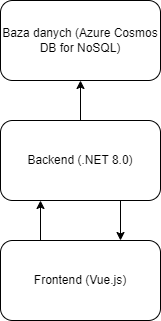
\includegraphics[width=0.2\linewidth]{img/architecture.drawio.png}
    \caption{Architektura aplikacji.}
\end{figure}

\subsection{Implementacja frontendu}
\indent Aplikacja frontend składa się z jednej strony, której zawartość zmienia się w zależności od wyborów gracza. Przed rozpoczęciem rozgrywki, gracz może wybrać zasady - czy statki mogą się ze sobą stykać. Dropdown z wyborem algorytmu przeciwnika jest dostępny jedynie w lokalnie zbudowanej wersji aplikacji. Wersja produkcyjna, dostępna dla graczy nie daje takiego wyboru. Dzięki temu gracze nie wiedzą z jakim algorytmem grają podczas rozstawiania swoich statków, nie wiedzą więc jakie rozstawienie najbardziej by im się opłaciło.

Dostępne są dwie wersje językowe aplikacji - polska oraz angielska.

\begin{figure}[!h]
    \label{fig:frontend-start}
    \centering 
\includegraphics[width=1\linewidth]{img/frontend-start.PNG}
    \caption{Aplikacja frontend przed rozpoczęciem rozgrywki}
\end{figure}

Po kliknięciu 'Rozpocznij grę', gracz widzi przed sobą dwie plansze, tak jak przedstawia to rysunek 4.2. Na górze znajduje się plansza przeciwnika, z niewidocznymi statkami, na dole zaś znajduje się plansza gracza, na której musi rozmieścić swoje statki. W tym celu użytkownik może skorzystać z przycisków znajdujących się pod swoją planszą. Rozwiązanie to zapewnia możliwość gry również na urządzeniach mobilnych, gdzie korzystanie ze strzałek na klawiaturze byłoby problematyczne.

\indent Na górze strony znajduje się element przedstawiający obecny stan gry - na rysunku 4.2 widnieje na nim 'Czekanie na rozmieszczenie statków przez użytkownika'. Ma to na celu zapewnienie graczowi informacji, co ma teraz robić.

\begin{figure}[!h]
    \label{fig:frontend-game}
    \centering 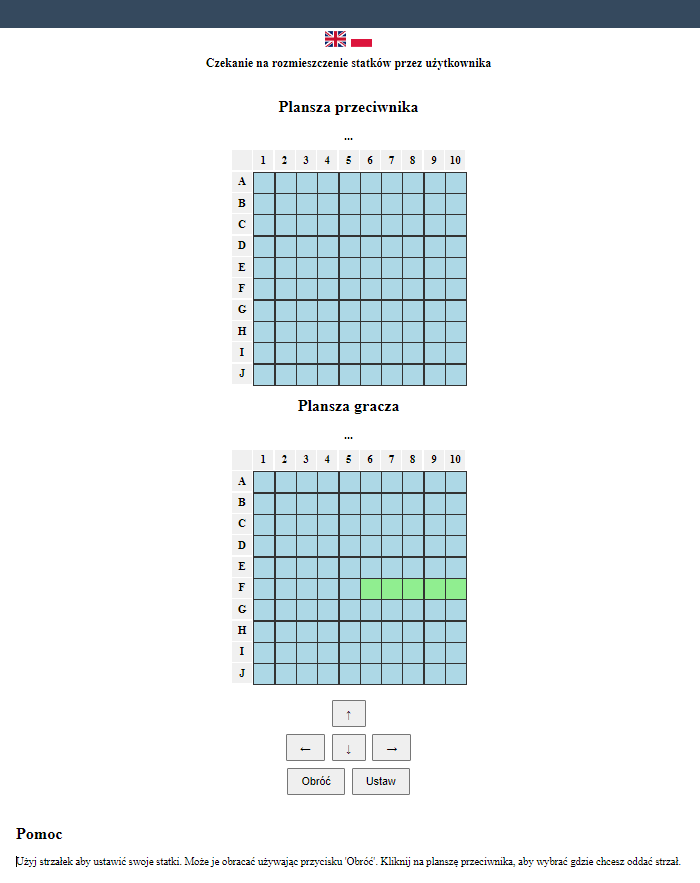
\includegraphics[width=1\linewidth]{img/frontend-game.PNG}
    \caption{Aplikacja frontend na starcie rozgrywki}
\end{figure}

Po rozstawieniu statków rozpoczyna się właściwa rozgrywka. Gracz i przeciwnik na zmianę oddają strzały, a nad ich planszami widać informację zwrotną o ostatnim strzale. Aby oddać strzał, gracz musi jedynie kliknąć daną komórkę na planszy przeciwnika. Gra kończy się gdy wszystkie statki jednej ze stron zostaną zatopione. 

\begin{figure}[!h]
    \label{fig:frontend--in-game}
    \centering 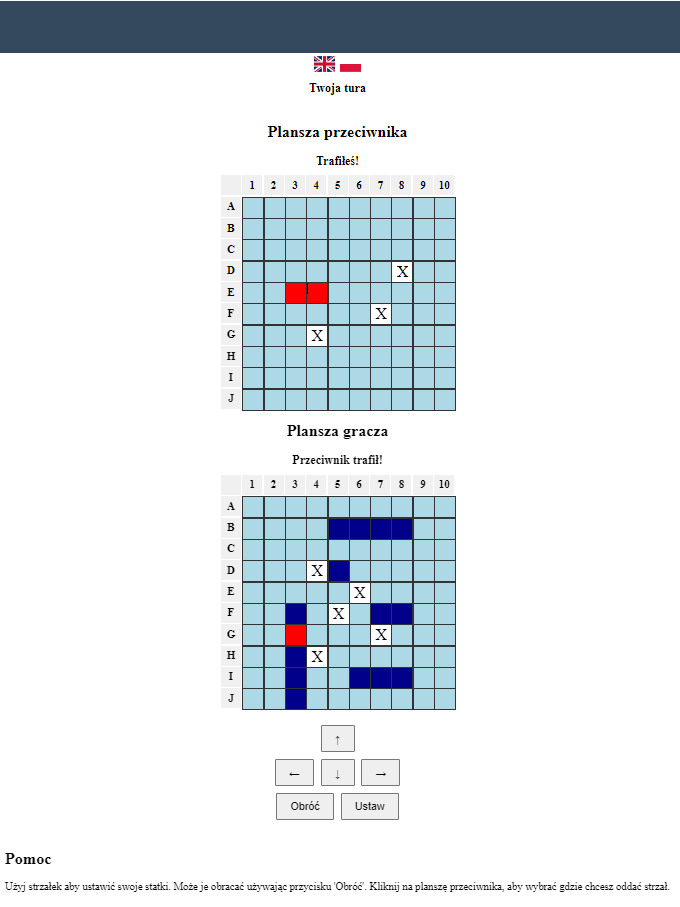
\includegraphics[width=1\linewidth]{img/frontend-in-game.PNG}
    \caption{Aplikacja frontend w trakcie rozgrywki}
\end{figure}

Aplikacja frontend składa się jedynie z kilku komponentów:
\begin{itemize}
    \item \textbf{Header.vue}: Tytuł strony "Statki", widoczny na rysunku 4.1.
    \item \textbf{Help.vue}: Wskazówki dla gracza, widoczne na dole rysunków 4.1, 4.2 i 4.3.
    \item \textbf{Menu.vue}: Menu z wyborem heurystyki oraz zasad, widoczne na rysunku 4.1.
    \item \textbf{OpponentGrid.vue}: Plansza przeciwnika, widoczna na rysunkach 4.2 i 4.3.
    \item \textbf{UserGrid.vue}: Plansza gracza, widoczna na rysunkach 4.2 i 4.3.
\end{itemize}

Plansze gracza i przeciwnika są oddzielnymi elementami, ponieważ różnią się zaimplementowaną logiką. Plansza przeciwnika przedstawia jedynie informacje płynące z backendu o tym które pole zostało trafione i w które już strzelaliśmy. Plansza gracza zaś zapewnia możliwość rozstawienia statków. Z powyższych elementów korzysta główny komponent aplikacji, plik App.vue.

Kluczowy jest też plik GameApi.js, w którym zdefiniowany jest klient API oraz endpointy, które wołane są po stronie backendu.

Po otwarciu aplikacji na nowej przeglądarce zapisywany jest plik cookie 'sessionId', który następnie wysyłany jest z każdym zapytaniem do API. W ten sposób backend wie, który gracz woła API i na tej podstawie aktualizuje stan danej gry. Projekty Web API w technologii .NET zapewniają podobną funkcjonalność, ale niestety, aby z niej skorzystać użytkownik musi wyrazić zgodę na 'Pliki cookie innych firm' w przeglądarce. 

\subsection{Implementacja backendu}
\indent Aplikacja składa się z kilku projektów:
\begin{itemize}
    \item \textbf{Battleships.AI}: Zawiera heurystyki wykorzystywane do podejmowania decyzji przez przeciwnika.
    \item \textbf{Battleships.Common}: Zawiera klasy wykorzystywane w pozostałych projektach.
    \item \textbf{Battleships.Core}: Zawiera kluczowe dla aplikacji serwisy.
    \item \textbf{Battleships.UnitTests}: Zawiera testy jednostkowe, które zostały wykorzystane do testowania, która heurystyka jest najskuteczniejsza.
    \item \textbf{Battleships.WebApi}: RESTful API, które komunikuje się z frontendem. Zawiera kontrolery, do których wstrzyknięte za pomocą DI (Dependency injection) zostały serwisy z projektu Battleships.Core.
\end{itemize}

Endpointy, które zapewnia Battleships.WebApi.
\begin{itemize}
    \item \textbf{POST /api/AiType/list}: Zwraca listę algorytmów dostępnych do wyboru. Jest to endpoint typu POST, ponieważ do backendu przesyłana jest informacja jakie zasady wybrał gracz - czy statki mogą się ze sobą stykać. Używany na lokalnym środowisku.
    \item \textbf{POST /api/AiType/select}: Umożliwia graczowi wybór algorytmu decyzyjnego przeciwnika. Używany jedynie na lokalnym środowisku.
    \item \textbf{GET /api/GameState/get}: Zwraca obecny stan rozgrywki, a więc rozmieszczenie statków obu stron oraz dotychczasowe strzały.
    \item \textbf{GET /api/GameState/clear}: Umożliwia wyczyszczenie dotychczasowego stanu gry. Endpoint ten jest wołany po otwarciu gry, aby wyczyścić dotychczasową rozgrywkę - w ten sposób unikamy nieprzewidzianego zachowania aplikacji.
    \item \textbf{POST /api/Rules/update}: Umożliwia wybór zasad - czy statki mogą się ze sobą stykać.
    \item \textbf{POST /api/ShipLocations/user}: Umożliwia rozmieszczenie statków graczowi. Endpoint ten jest wołany gdy użytkownik rozstawi wszystkie 5 swoich statków.
    \item \textbf{GET /api/ShipLocations/opponent}: Zwraca rozmieszczenie statków przeciwnika.
    \item \textbf{POST /api/Shot/user}: Umożliwia użytkownikowi oddanie strzału, wołany jest za każdym razem gdy użytkownik w swojej turze wybierze komórkę na planszy przeciwnika.
    \item \textbf{GET /api/Shot/opponent}: Zwraca komórkę, którą algorytm decyzyjny przeciwnika wybrał do ostrzału.
\end{itemize}

Dokumentacja API dostępna jest pod adresem \url{https://battleshipswebapi.azurewebsites.net/swagger/index.html}.
\newline \newline
Najważniejszą klasą jest GameState, widoczna na listingu 1. Wykorzystywana ona jest za każdym razem, gdy algorytm decyzyjny kalkuluje najbardziej korzystny z punktu widzenia danej heurystyki ruch. Dalej opisane zostaną klasy wykorzystane w GameState. Klasa Ship, widoczna na listingu 2, opisuje rozmiar, położenie oraz status statku. Klasa shot, widoczna na listingu 3, opisuje dany strzał - w jakie pole został oddany, oraz czy trafiony został jakiś statek. Enum AiType określa rodzaj heurystyki.

PlayerAiType jest domyślnie puste, ponieważ w trakcie rozgrywki gracz-przeciwnik, to gracz podejmuje decyzje odnośnie strzałów. Pole to jest wykorzystywane jedynie w testach jednostkowych, gdzie jako gracz występuje algorytm decyzyjny.
\begin{addmargin}[10mm]{0mm}
\begin{lstlisting}[
    language={[Sharp]C},
    numbers=left,
    firstnumber=5,
    caption={Klasa GameState},
    aboveskip=0pt
]
public class GameState
{
    public List<Ship> UserShips { get; set; } = [];
    public List<Ship> OpponentShips { get; set; } = [];
    public List<Shot> PlayerShots { get; set; } = [];
    public List<Shot> OpponentShots { get; set; } = [];
    public AiType? PlayerAiType { get; set; } = null;
    public AiType OpponentAiType { get; set; }
    public bool ShipsCanTouch { get; set; }
}
\end{lstlisting}
\end{addmargin}

\begin{addmargin}[10mm]{0mm}
\begin{lstlisting}[
    language={[Sharp]C},
    numbers=left,
    firstnumber=3,
    caption={Klasa Ship},
    aboveskip=0pt
]
public class Ship
{
    public int Size { get; set; }
    public List<Coordinate> Coordinates { get; set; } = [];
    public bool IsSunk { get; set; } = false;
}
\end{lstlisting}
\end{addmargin}

\begin{addmargin}[10mm]{0mm}
\begin{lstlisting}[
    language={[Sharp]C},
    numbers=left,
    firstnumber=3,
    caption={Klasa Shot},
    aboveskip=0pt
]
public class Shot
{
    public int X { get; set; }
    public int Y { get; set; }
    public bool IsHit { get; set; }
}
\end{lstlisting}
\end{addmargin}

\begin{addmargin}[10mm]{0mm}
\begin{lstlisting}[
    language={[Sharp]C},
    numbers=left,
    firstnumber=3,
    caption={Enum AiType},
    aboveskip=0pt
]
public class Shot
public enum AiType
{
    Random = 0,
    RandomPlus = 1,

    LocationHeuristic = 2,
    LocationHeuristicDynamic = 3,
    HitHeuristic = 4,
    LocationAndHitHeuristic = 5,
    LocationAndHitHeuristicDynamic = 6,
}
\end{lstlisting}
\end{addmargin}

\subsection{Implementacja algorytmów decyzyjnych}
\indent Algorytmy decyzyjne w projekcie zostały zaimplementowane jedynie dla fazy gry, w której oddawane są strzały. Statki przeciwnika rozstawiane są zawsze losowo na planszy. W poniższym rozdziale wypisane zostały fragmenty kodu na najwyższym poziomie abstrakcji, bardziej dokładna analiza znajduje się w załączniku 1.

Wszystkie algorytmy są implementacją interfejsu IAiStrategy, przedstawionego na listingu 5.

\begin{addmargin}[10mm]{0mm}
\begin{lstlisting}[
    language={[Sharp]C},
    numbers=left,
    firstnumber=1,
    caption={Interfejs IAiStrategy},
    aboveskip=0pt
]
using Battleships.Common.GameClasses;

namespace Battleships.AI.Strategies
{
    public interface IAiStrategy
    {
        (int X, int Y) GenerateMove(
            List<Shot> previousShots,
            List<Ship> opponentShips,
            bool shipsCanTouch);
    }
}
\end{lstlisting}
\end{addmargin}

Algorytmy korzystające z heurystyk, dodatkowo dziedziczą po abstrakcyjnej klasie HeuristicStrategyBase, przedstawionej na listingu 6. Każdy taki algorytm musi implementować metodę GenerateProbabilityMap. Generowana przez tę metodę mapa prawdopodobieństwa określa jak duża jest szansa (według danej heurystyki) że na danej komórce znajduje się statek. Mapa jest listą par liczb (A,B), gdzie A określa współrzędne komórki, a B prawdopodobieństwo wystąpienia statku. W tym kontekście słowo 'prawdopodobieństwo' jest używane potocznie, a liczba B nie jest równa dokładnemu prawdopodobieństwu. Każda z heurystyk ma różne wagi, i oblicza liczbę B na inny sposób, korzystając z umownych wartości.

\indent Na podstawie wygenerowanej mapy prawdopodobieństwa, algorytm wybiera najbardziej korzystny ruch. 

\begin{addmargin}[10mm]{0mm}
\begin{lstlisting}[
    language={[Sharp]C},
    numbers=left,
    firstnumber=9,
    caption={Abstrakcyjna klasa HeuristicStrategyBase},
    aboveskip=0pt
]
public abstract class HeuristicStrategyBase
    : IAiStrategy
{
    private static readonly Random _random = new();

    public (int X, int Y) GenerateMove(
        List<Shot> previousShots,
        List<Ship> opponentShips,
        bool shipsCanTouch)
    {
        var probabilityMap = GenerateProbabilityMap(
            previousShots,
            opponentShips,
            shipsCanTouch);

        var maxProbability = probabilityMap.Max();

        List<(int, int)> bestMoves = probabilityMap
            .Select((prob, index) => (prob, index))
            .Where(x => x.prob == maxProbability)
            .Select(x => (x.index % 10, x.index / 10))
            .Where(x => !previousShots
                .Any(shot => shot.X == x.Item1
                    && shot.Y == x.Item2))
            //make sure we're not shooting at
            //the same cell twice
            .ToList();

        if (bestMoves.Count != 0)
        {
            var move = bestMoves[_random.Next(bestMoves.Count)];
            return move;
        }

        // Fallback to a random move if no valid moves found
        // (shouldn't happen with a 10x10 grid)
        return new RandomStrategy().GenerateMove(
            previousShots,
            opponentShips,
            shipsCanTouch);
    }

    public abstract int[] GenerateProbabilityMap(
        List<Shot> previousShots,
        List<Ship> opponentShips,
        bool shipsCanTouch);
}
\end{lstlisting}
\end{addmargin}

\subsubsection{Algorytm losowy}
Najprostszy algorytm, w trakcie implementacji był traktowany jako grupa kontrolna - jeśli dany algorytm miał niższą skuteczność od algorytmu losowego, to coś z nim było nie tak. Jedynym ograniczeniem przy wybieraniu komórki do ostrzału jest to, czy nie oddano już w nią strzału wcześniej.

\subsubsection{Rozszerzony algorytm losowy}
Dostępny jedynie gdy gracz wybierze opcję 'statki nie mogą się ze sobą stykać'. Różni się od zwykłego algorytmu losowego tym, że pomijane są pola, które sąsiadują z zatopionymi statkami.

\subsubsection{Algorytm oparty na heurystyce maksymalizacji zysku ze strzału}
Widoczny jest na listingu 7. Metoda AdjustProbabilityForShipLocations dla każdego niezatopionego statku przeciwnika iteruje przez całą planszę i sprawdza czy początek statku może rozpoczynać się na danej komórce. Jako początek statku traktujemy jego współrzędną o najmniejszych współrzędnych X i Y. Możliwe położenie statku jest analizowane zarówno w pionie jak i poziomie. Warunkami, które wykluczają możliwość rozpoczęcia się statku na danej komórce to:
\begin{itemize}
    \item (Jeśli użytkownik zaznaczył opcję 'statki nie mogą się ze sobą stykać.) Jakakolwiek komórka sąsiadująca z możliwymi współrzędnymi statku została trafiona - czyli leży na niej inny statek przeciwnika.
    \item Jakakolwiek komórka będąca możliwą współrzędną statku została już wcześniej ostrzelana.
    \item Jakakolwiek komórka będąca możliwą współrzędną statku została już wcześniej trafiona i jest częścią zatopionego statku.
\end{itemize}
Jeśli przykładowo statek o długości L może rozpoczynać się na komórce (X,Y) i leżeć w poziomie, to na mapie prawdopodobieństwa dodajemy liczbę 1 do komórek (X,Y), ..., (X+L, Y).


Metody AdjustProbabilityForSunkShips oraz AdjustProbabilityForShotAtCells są wykorzystywana również w pozostałych algorytmach opartych na heurystykach - służą ona do wyzerowania wartości na mapie prawdopodobieństwa dla komórek, które zostały już ostrzelane lub sąsiadują z zatopionymi statkami (jeśli statki nie mogą się ze sobą stykać według zasad).

\begin{addmargin}[10mm]{0mm}
\begin{lstlisting}[
    language={[Sharp]C},
    numbers=left,
    firstnumber=9,
    caption={Klasa LocationHeuristicStrategy},
    aboveskip=0pt
]
public class LocationHeuristicStrategy
    : HeuristicStrategyBase
{
    private readonly static int
        POSSIBLE_SHIP_LOCATION_WEIGHT = 1;

    public override int[] GenerateProbabilityMap(
        List<Shot> previousShots,
        List<Ship> opponentShips,
        bool shipsCanTouch)
    {
        var probabilityMap = new int[100];

        HeuristicHelper.AdjustProbabilityForShipLocations(
            previousShots,
            opponentShips,
            shipsCanTouch,
            probabilityMap,
            POSSIBLE_SHIP_LOCATION_WEIGHT);

        if (!shipsCanTouch)
        {
            HeuristicHelper.AdjustProbabilityForSunkShips(
            opponentShips,
            probabilityMap);
        }

        HeuristicHelper.AdjustProbabilityForShotAtCells(
            previousShots,
            probabilityMap);

        GridHelper.PrintProbabilityGrid(probabilityMap, 10, 10);
        // just for debugging purposes

        return probabilityMap;
    }
}

\end{lstlisting}
\end{addmargin}

\subsubsection{Algorytm oparty na heurystyce najbardziej prawdopodobnej lokalizacji na podstawie trafień}
Algorytm jest widoczny na listingu 8. Metoda AdjustProbabilityForHitClusters znajduje dotychczasowe trafienia, które nie należą do zatopionych statków. W przypadku pojedynczych trafień, zwiększone zostają wartości na mapie prawdopodobieństwa dla komórek sąsiadujących w poziomie i w pionie z trafioną komórką. Jeśli znaleziona zostaje seria sąsiadujących trafień, zwiększone są wartości prawdopodobieństwa dla sąsiadujących komórek, znajdujących się na przedłużeniu tej serii. Wartość dodawana w tym przypadku ma większą wartość niż dla pojedynczych trafień.

\begin{addmargin}[10mm]{0mm}
\begin{lstlisting}[
    language={[Sharp]C},
    numbers=left,
    firstnumber=9,
    caption={Klasa HitHeuristicStrategy},
    aboveskip=0pt
]
public class HitHeuristicStrategy : HeuristicStrategyBase
{
    private readonly static int
        NEXT_TO_A_SINGLE_HIT_WEIGHT = 50,
        IN_LINE_WITH_OTHER_HITS_WEIGHT = 100;

    public override int[] GenerateProbabilityMap(
        List<Shot> previousShots,
        List<Ship> opponentShips,
        bool shipsCanTouch)
    {
        var probabilityMap = new int[100];

        HeuristicHelper.AdjustProbabilityForHitClusters(
            previousShots,
            opponentShips,
            probabilityMap,
            NEXT_TO_A_SINGLE_HIT_WEIGHT,
            IN_LINE_WITH_OTHER_HITS_WEIGHT);

        if (shipsCanTouch)
        {
            HeuristicHelper.AdjustProbabilityForSunkShips(
                opponentShips,
                probabilityMap);
        }

        HeuristicHelper.AdjustProbabilityForShotAtCells(
            previousShots,
            probabilityMap);

        GridHelper.PrintProbabilityGrid(probabilityMap, 10, 10);
        // just for debugging purposes

        return probabilityMap;
    }
}

\end{lstlisting}
\end{addmargin}

\subsubsection{Algorytm oparty na heurystyce maksymalizacji zysku priorytetyzującej dłuższe statki}
Właściwie identyczny do algorytmu opisanego w rozdziale 4.5.3. Jedyną różnicę pomiędzy algorytmami widać na listingu 9. Dla tego algorytmu zmienna dynamicWeight równa jest TRUE, a więc jeśli statek może znajdować się na danej komórce, to zamiast dodawać do niego zwykłą wagę, dodajemy wagę przemnożoną przez długość statku do potęgi dynamicPower (w tym przypadku 2). Wzór ten został już wspomniany w rozdziale 3.4, w punkcie 3.

\begin{addmargin}[10mm]{0mm}
\begin{lstlisting}[
    language={[Sharp]C},
    numbers=left,
    firstnumber=24,
    caption={Zwiększanie wartości na mapie prawdopodobieństwa dla algorytm oparty na heurystyce maksymalizacji zysku priorytetyzującej dłuższe statki},
    aboveskip=0pt
]
probabilityMap[(y * 10) + x + i] += dynamicWeight
    ? weight * (int)Math.Pow(length, dynamicPower)
    : weight;
\end{lstlisting}
\end{addmargin}

\subsubsection{Algorytm oparty na heurystykach maksymalizacji zysku oraz najbardziej prawdopodobnej lokalizacji na podstawie trafień}
Kombinacja algorytmów z punktów 4.5.3 i 4.5.4. Znacznie większą wagę ma tu heurystyka najbardziej prawdopodobnej lokalizacji na podstawie trafień, a więc w praktyce heurystyka maksymalizacji zysku spełnia w pewnym sensie funkcję pomocniczą - wskazuje cele, jeśli żadna komórka nie została jeszcze trafiona, lub rozstrzyga, w którą z wielu komórek sąsiadujących z trafieniami najbardziej opłaca się strzelić, aby wyeliminować najwięcej możliwych położeń statków. Wszystkie metody widoczne w listingu 10 zostały opisane już we wcześniejszych punktach.

\begin{addmargin}[10mm]{0mm}
\begin{lstlisting}[
    language={[Sharp]C},
    numbers=left,
    firstnumber=10,
    caption={Klasa LocationAndHitHeuristicStrategy},
    aboveskip=0pt
]
    public class LocationAndHitHeuristicStrategy : HeuristicStrategyBase
    {
        private readonly static int
            POSSIBLE_SHIP_LOCATION_WEIGHT = 1,
            NEXT_TO_A_SINGLE_HIT_WEIGHT = 50,
            IN_LINE_WITH_OTHER_HITS_WEIGHT = 100;

        public override int[] GenerateProbabilityMap(
            List<Shot> previousShots,
            List<Ship> opponentShips,
            bool shipsCanTouch)
        {
            var probabilityMap = new int[100];

            HeuristicHelper.AdjustProbabilityForShipLocations(
                previousShots, opponentShips,
                shipsCanTouch,
                probabilityMap,
                POSSIBLE_SHIP_LOCATION_WEIGHT);

            HeuristicHelper.AdjustProbabilityForHitClusters(
                previousShots,
                opponentShips,
                probabilityMap,
                NEXT_TO_A_SINGLE_HIT_WEIGHT,
                IN_LINE_WITH_OTHER_HITS_WEIGHT);

            if (!shipsCanTouch)
            {
                HeuristicHelper.AdjustProbabilityForSunkShips(
                    opponentShips,
                    probabilityMap);
            }

            HeuristicHelper.AdjustProbabilityForShotAtCells(
                previousShots,
                probabilityMap);

            GridHelper.PrintProbabilityGrid(probabilityMap, 10, 10);
            // just for debugging purposes

            return probabilityMap;
        }
    }
\end{lstlisting}
\end{addmargin}

\subsubsection{Algorytm oparty na heurystykach maksymalizacji zysku oraz najbardziej prawdopodobnej lokalizacji na podstawie trafień priorytetyzującej dłuższe statki}
Bardzo podobna do punktu 4.5.6, z jedną różnicą - jeśli na planszy przeciwnika nie ma żadnego trafienia nienależącego do zatopionego statku, zamiast zwykłej heurystyki maksymalizacji zysku, stosujemy heurystykę maksymalizacji zysku priorytetyzującą dłuższe statki.

\begin{addmargin}[10mm]{0mm}
\begin{lstlisting}[
    language={[Sharp]C},
    numbers=left,
    firstnumber=10,
    caption={Klasa LocationAndHitHeuristicDynamicStrategy},
    aboveskip=0pt
]
public class LocationAndHitHeuristicDynamicStrategy
    : HeuristicStrategyBase
{
    private readonly static int
        POSSIBLE_SHIP_LOCATION_WEIGHT = 1,
        NEXT_TO_A_SINGLE_HIT_WEIGHT = 50,
        IN_LINE_WITH_OTHER_HITS_WEIGHT = 100;

    public override int[] GenerateProbabilityMap(
        List<Shot> previousShots,
        List<Ship> opponentShips,
        bool shipsCanTouch)
    {
        var probabilityMap = new int[100];

        var clusterCount =
        HeuristicHelper.AdjustProbabilityForHitClusters(
            previousShots,
            opponentShips,
            probabilityMap,
            NEXT_TO_A_SINGLE_HIT_WEIGHT,
            IN_LINE_WITH_OTHER_HITS_WEIGHT);

        if (clusterCount == 0)
        {
            HeuristicHelper.AdjustProbabilityForShipLocations(
                previousShots, opponentShips,
                shipsCanTouch,
                probabilityMap,
                POSSIBLE_SHIP_LOCATION_WEIGHT,
                dynamicWeight: true,
                dynamicPower: 2);
        }
        else
        {
            HeuristicHelper.AdjustProbabilityForShipLocations(
                previousShots,
                opponentShips,
                shipsCanTouch,
                probabilityMap,
                POSSIBLE_SHIP_LOCATION_WEIGHT);
        }

        if (!shipsCanTouch)
        {
            HeuristicHelper.AdjustProbabilityForSunkShips(
                opponentShips,
                probabilityMap);
        }

        HeuristicHelper.AdjustProbabilityForShotAtCells(
            previousShots,
            probabilityMap);

        GridHelper.PrintProbabilityGrid(probabilityMap, 10, 10);
        // just for debugging purposes

        return probabilityMap;
    }
}
\end{lstlisting}
\end{addmargin}
\indent
\newpage % Rozdziały zaczynamy od nowej strony.
\section{Przegląd istniejących rozwiązań}

\subsection{Analiza literatury}
Tematyka tej pracy została już poruszana w wielu pracach i artykułach naukowych. Poniżej zostaną one opisane oraz przeanalizowane zostaną podobieństwa i różnice.

\subsubsection{Efficient Algorithms for Battleship \cite{crombez2020efficient}}
Praca ta analizuje algorytmiczny problem, pojawiający się w grze statki, a mianowicie jak zatopić trafiony statek w jak najmniejszej liczbie ruchów. W założeniach pracy występuje szereg uproszczeń:
\begin{itemize}
    \item Flota ostrzeliwana przez algorytm składa się z tylko jednego statku.
    \item Jedna ze współrzędnych statku przeciwnika jest już znana.
    \item Statki nie mogą być obracane - zawsze znana jest orientacja statku.
\end{itemize}
Praca analizuje za to szerszy wachlarz kształtów statków. Rozważane są przypadki:
\begin{enumerate}
    \item Współrzędne ułożone w linii prostej.
    \item Współrzędne niezawierające równoległoboków.
    \item Współrzędne składające się z poziomo-pionowo wypukłych poliminów.
    \item Współrzędne składające się z cyfrowych zbiorów wypukłych.
\end{enumerate}

Przypadek nr 1 jest w przypadku tej pracy najbardziej trywialny, ale interesuje nas najbardziej z punktu widzenia niniejszej pracy magisterskiej. Pozostałe rodzaje kształtów wymagają zastosowania znacznie bardziej skomplikowanych algorytmów do znalezienia potencjalnych lokalizacji współrzędnych trafionego statku.
Algorytm zaproponowany dla przypadku nr. 1 to: po udanym trafieniu w komórkę (X,Y), należy strzelać w kolejne pola (X+1,Y),(X+2,Y),... aż spudłujemy. Jeśli statek rozpoczyna się w narożniku planszy (0,0), niemożliwe jest spudłowanie. Jeśli statek rozpoczyna się w innym miejscu, możliwe jest jednokrotne spudłowanie, po czym należy zacząć ostrzeliwać komórki po drugiej stronie (X,Y), tj. (X-1,Y), (X-2,Y),... . Maksymalna liczba spudłowań według tego algorytmu to 1.

Podobna logika została zaimplementowana w algorytmie opartym na heurystyce najbardziej prawdopodobnej lokalizacji na
podstawie trafień z rozdziału 4.5.4. Nasz przypadek jest jednak trochę bardziej skomplikowany, ponieważ nie jest znana orientacja statku, a floty składają się zawsze z 5 statków. Oto działanie naszego algorytmu w podobnej sytuacji - kiedy znamy jedną współrzędną statku (X,Y).

\begin{itemize}
\item Rozważymy uproszczony przypadek, tj. nie oddano jeszcze żadnych strzałów poza tym, który trafił w jedną ze współrzędnych statku. W takiej sytuacji komórki, które wskaże nasz algorytm to poziomi i pionowi sąsiedzi (X,Y). W najlepszym przypadku, czyli kiedy (X,Y) znajduje się w narożniku planszy, istnieją jedynie 2 takie komórki. Algorytm może spudłować jedynie raz, zanim trafi kolejną komórkę i tym samym zdobędzie informację o orientacji statku. Mając te informację, może zatopić statek, nie pudłując już ani razu.

\item W bardziej pesymistycznym scenariuszu, gdy (X,Y)) znajduje się na środku planszy, algorytm będzie ostrzeliwał po kolei 4 sąsiadujące komórki, aż w którąś trafi. Możliwe jest więc że spudłuje 3 razy zanim zdobędzie informację o orientacji statku. Po ustaleniu orientacji, algorytm ostrzeliwuje sąsiadujące komórki leżące na przedłużeniu serii trafień. Jeśli w pierwszym kroku spudłowano 3 razy, to istnieje już jedynie 1 taka komórka, a więc nie możemy spudłować w kroku drugim. Zatem maksymalna liczba spudłowań to 3.
\end{itemize}

Po rozważeniu obu przypadków, maksymalna liczba spudłowań dla naszego algorytmu to 3.


\subsubsection{Developing a Heuristic via Diagrammatic Reasoning \cite{anderson1995developing}}

Autorzy pracy opisują korzyści nadania komputerom umiejętnośći rozumowania za pomocą diagramów. Opisują między innymi metodę intra-diagramatycznego rozumowania (Intra-diagrammatic reasoning) i pokazują jej użyteczność do stworzenia prostej heurystyki do gry w statki. Opisywana metoda polega na aplikowaniu różnych operatorów do pojedynczego diagramu, między innymi:
\begin{itemize}
    \item Przypisanie
    \item Negacja
    \item Suma logiczna
    \item Iloraz logiczny
\end{itemize}

Zasady gry Statki przyjęte w tej pracy różnią się trochę od tych wcześniej opisywanych w rozdziale 2.2 - autorzy założyli że statki mogą być ustawione również na skos, jednak sama metoda wnioskowania jest bardzo zbliżona do tych użytych w opisywanej pracy magisterskiej. Dodatkowym założeniem jest to, że flota składa się jedynie z jednego pięciomasztowca, a gracze co turę oddają 'salwę' siedmiu strzałów.

Prawdopodobieństwo wystąpienie na danej komórce statku jest determinowane w następujący sposób: tworzone są 4 diagramy o wymiarach 10 na 10, po jednym dla każdej możliwej orientacji statku. Na każdy z diagramów 'nakładane' są możliwe pozycje statków w danej orientacji. Każde takie 'nałożenie' statku na diagram powoduje zaciemnienie komórek, które są jego potencjalnym położeniem. Tak więc komórki na których może leżeć kilka różnych wariantów statku są ciemniejsze od pozostałych. Dla przykładu, jeśli rozważamy dwie możliwe lokalizacje statku:
\begin{itemize}
    \item Pomiędzy komórkami (0,0) i (4,0)
    \item Pomiędzy komórkami (1,0) i (5,0)
\end{itemize}
To na wynikowym diagramie komórki (0,0) oraz (5,0) będą jaśniejsze od pozostałych.

4 diagramy otrzymane w ten sposób nakładamy na siebie i otrzymujemy diagram A mapę prawdopodobieństwa wystąpienia statku. Na podstawie tej mapy wybrane zostają komórki, które zostaną ostrzelane w kolejnej turze. Jeśli jakieś komórki zostały już ostrzelane wcześniej, dodajemy je do diagramu B. Aby otrzymać ostateczną mapę prawdopodobieństwa, stosujemy operację
\begin{align*}
    A \land \neg B
\end{align*}

W ten sposób eliminujemy z rozważań komórki, które zostały już ostrzelane. Metoda ta w swoim założeniu jest identyczna do heurystyki maksymalizacji zysku ze strzału opisanej w rozdziale 3.4.


\newpage % Rozdziały zaczynamy od nowej strony.
\section{Analiza skuteczności algorytmów}

\subsection{Metody testowania}
\indent\ Testy zostały przeprowadzone za pomocą testów jednostkowych, w których wszystkie algorytmy zostały zestawione przeciwko sobie. Statki były rozstawione losowo dla obu stron. Wszystkie testy jednostkowe dziedziczą po klasie bazowej AlgorithmTestBase, która była potrzebna do inicjalizacji lub zmockowania wszelkich potrzebnych serwisów. Na listingu 12 widoczny jest przykładowy test jednostkowy. Testowane były oba warianty zasady stykania się statków. Stała numberOfIterations wynosiła 1000, więc dla każdego zestawienia algorytmów i zasad otrzymano 1000 wyników. Ogólnie podczas testów zebrano około 40 000 rekordów w kontenerze TestGameSessions.

\begin{addmargin}[10mm]{0mm}
\begin{lstlisting}[
    language={[Sharp]C},
    numbers=left,
    firstnumber=11,
    caption={Przykładowy test jednostkowy},
    aboveskip=0pt
]
[Fact]
public void VsRandomShipsCantTouch()
{
    _httpContextAccessor.SetupTestHttpContext();

    var initialGameState = new GameState
    {
        PlayerAiType = AiType.LocationHeuristic,
        OpponentAiType = AiType.Random,
        ShipsCanTouch = false,
    };

    var playerWins = TestHelper.RunSimulation(
        initialGameState,
        _gameStateService,
        _generateMoveService,
        _shipLocationService,
        numberOfIterations);

    Assert.True(true);
}
\end{lstlisting}
\end{addmargin}


\subsection{Wyniki testów algorytmów}
W tabelach widocznych w poniższych rozdziałach stosowane będą skrócone nazwy algorytmów, tak aby bez problemu mieściły się w komórkach tabel. Poniżej znajduje się objaśnienie skrótów.
\begin{itemize}
    \item \textbf{Max. zysk} - Algorytm oparty na heurystyce maksymalizacji zysku ze strzału.
    \item \textbf{Analiza trafień} - Algorytm oparty na heurystyce najbardziej prawdopodobnej lokalizacji na podstawie trafień.
    \item \textbf{Max. zysk rozszerzony} - Algorytm oparty na heurystyce maksymalizacji zysku priorytetyzującej dłuższe statki.
    \item \textbf{Max. zysk + analiza trafień} - Algorytm oparty na heurystykach maksymalizacji zysku oraz najbardziej prawdopodobnej lokalizacji na podstawie trafień.
    \item \textbf{Max. zysk rozszerzony + analiza trafień} - Algorytm oparty na heurystykach maksymalizacji zysku oraz najbardziej prawdopodobnej lokalizacji na podstawie trafień priorytetyzującej dłuższe statki. 
\end{itemize}

W tabelach przedstawiających skuteczność poszczególnych algorytmów posłużono się kolorami, w celu podkreślenia otrzymanych wartości:
\begin{itemize}
    \item Kolor zielony - wynik zdecydowanie lepszy, skuteczność powyżej 55\%
    \item Kolor żółty - wynik porównywalny, skuteczność pomiędzy 45\%-55\%
    \item Kolor czerwony - wynik zdecydowanie gorszy, skuteczność poniżej 45\%
\end{itemize}

\subsubsection{Algorytm losowy}

Algorytm losowy, zgodnie z przewidywaniami wypadł najgorzej w zestawieniu z innymi algorytmami. W tabeli 6.1 widać, że najwyższy procent zwycięstw jaki osiągnął to 13,1\% przeciwko algorytmowi losowemu rozszerzonemu. Wśród wyników można zaobserwować prawidłowość, że skuteczność delikatnie wzrasta w przypadku testów, gdzie statki mogą się stykać. Zgodnie z tym co zostało wspomniane pod koniec rozdziału 2.2, dodatkowe ograniczenie tego, jak mogą być rozstawione statki, ułatwia heurystykom analizę planszy przeciwnika. Gdy tego ograniczenia nie ma, gra staje się trochę bardziej losowa - chociaż nadal algorytmy oparte na heurystykach są znacznie skuteczniejsze od algorytmu losowego.

\begin{table}[!h]
    \centering
    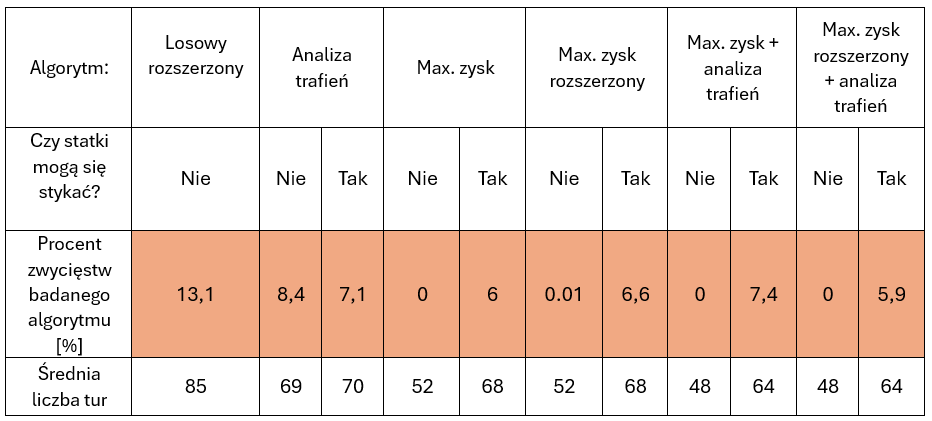
\includegraphics[width=1\linewidth]{img/table-random.png}
    \caption{Wyniki testów dla algorytmu losowego}
\end{table}

\subsubsection{Algorytm losowy z pominięciem pól sąsiadujących z zatopionymi statkami}

Algorytm losowy z pominięciem pól był testowany jedynie w przypadku gdy statki nie mogą się ze sobą stykać. W przeciwnym wypadku, gdyby oponent ustawił statki obok siebie, badany algorytm nie byłby w stanie odnieść zwycięstwa. W wynikach testów widocznych w tabeli 6.2 widać, że algorytm rozszerzony jest dużo skuteczniejszy od swojej podstawowej wersji. Można też zauważyć zdecydowany wzrost skuteczności przeciwko algorytmowi opartemu na heurystyce najbardziej prawdopodobnej lokalizacji na podstawie trafień. W pozostałych przypadkach również można zaobserwować wzrost skuteczności, ale jest on bardzo niewielki.
Test

\begin{table}[!h]
    \centering
    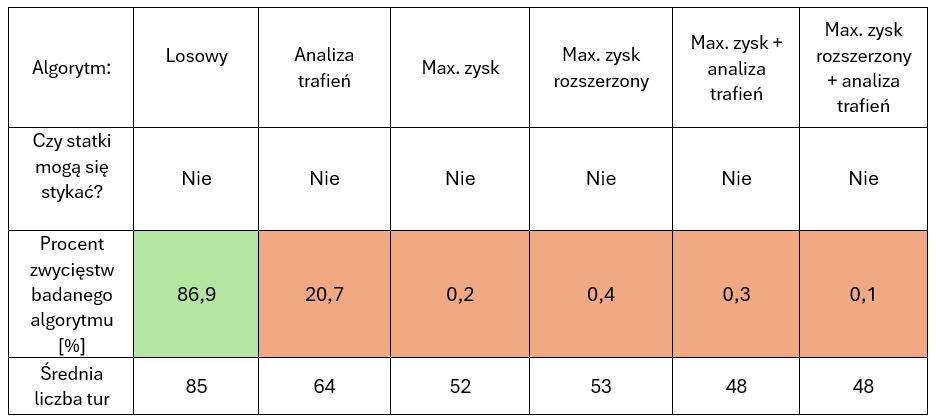
\includegraphics[width=1\linewidth]{img/table-random-plus.png}
    \caption{Wyniki testów dla algorytmu losowego rozszerzonego}
\end{table}

\subsubsection{Algorytm oparty na heurystyce najbardziej prawdopodobnej lokalizacji na podstawie trafień}

Jak widać w tabeli 6.3, w przypadku tego algorytmu widać wyraźnie jego przewagę nad algorytmami losowymi. Jest on jednak zdecydowanie najsłabszym z algorytmów heurystyczych. Umiejętność 'dobijania' trafionych statków wyróżnia go na tle algorytmów losowych, ale nadal jednak w dużej mierze opiera się na losowości - jeśli na planszy przeciwnika nie ma żadnego trafienia, algorytm oddaje strzały w losowe komórki.

Podobnie jak w 6.2.1, widać znaczące różnicę w zależności od wyboru zasad - skuteczność tego algorytmu wzrasta gdy statki mogą się ze sobą stykać.

\begin{table}[!h]
    \centering
    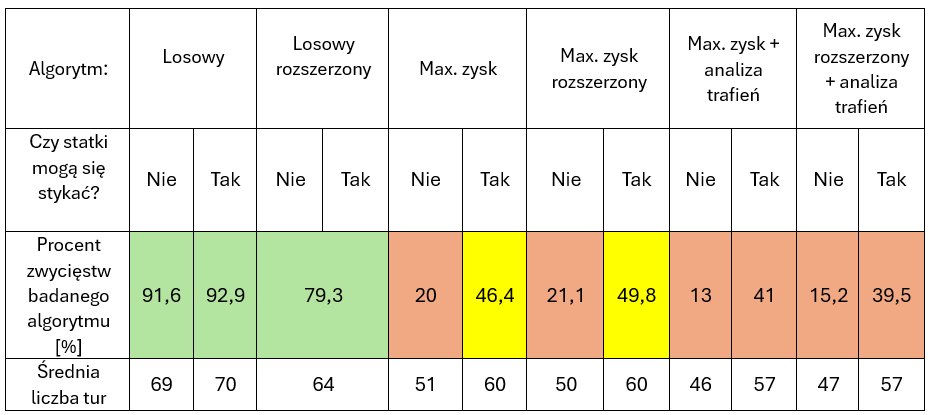
\includegraphics[width=1\linewidth]{img/table-hit-heuristic.png}
    \caption{Wyniki testów dla algorytmu opartego na heurystyce najbardziej prawdopodobnej lokalizacji na podstawie trafień}
\end{table}

\subsubsection{Algorytm oparty na heurystyce maksymalizacji zysku ze strzału}

Widać tu wzrost skuteczności o około 10\% względem względem algorytmów losowych. Algorytm jest też zdecydowanie skuteczniejszy od algorytmu opartego na heurystyce najbardziej prawdopodobnej lokalizacji na podstawie trafień, aczkolwiek gdy statki mogą się ze sobą stykać to ich skuteczność jest porównywalna.

\begin{table}[!h]
    \centering
    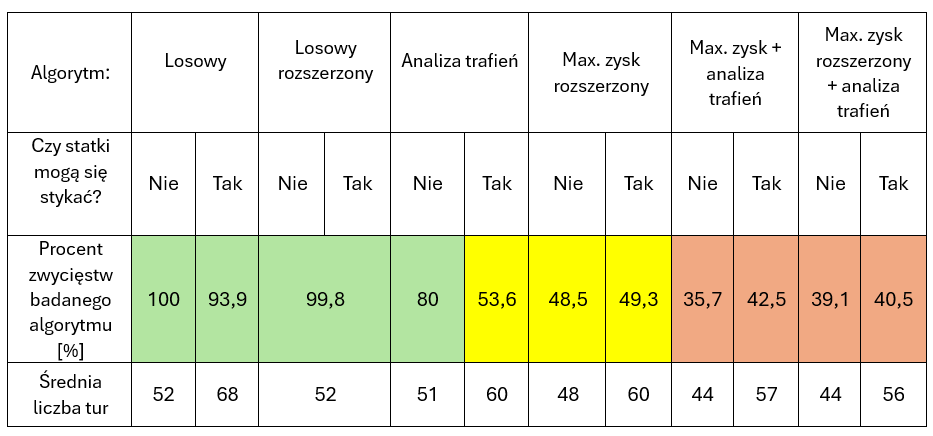
\includegraphics[width=1\linewidth]{img/table-location-heuristic.png}
    \caption{Wyniki testów dla algorytmu opartego na heurystyce maksymalizacji zysku ze strzału}
\end{table}


\subsubsection{Algorytm oparty na heurystyce maksymalizacji zysku priorytetyzującej dłuższe statki}

Wyniki są widoczne w tabeli 6.5 i są bardzo zbliżone do wartości z punktu 6.2.4. Można zaobserwować, że w bezpośrednim starciu, badany algorytm jest nieznacznie skuteczniejszy od swojego podstawowego wariantu. Jednak we wszystkich pozostałych przypadkach poza jednym widoczny jest nieznaczny spadek skuteczności, w najgorszym przypadku 3,5\%.

\begin{table}[!h]
    \centering
    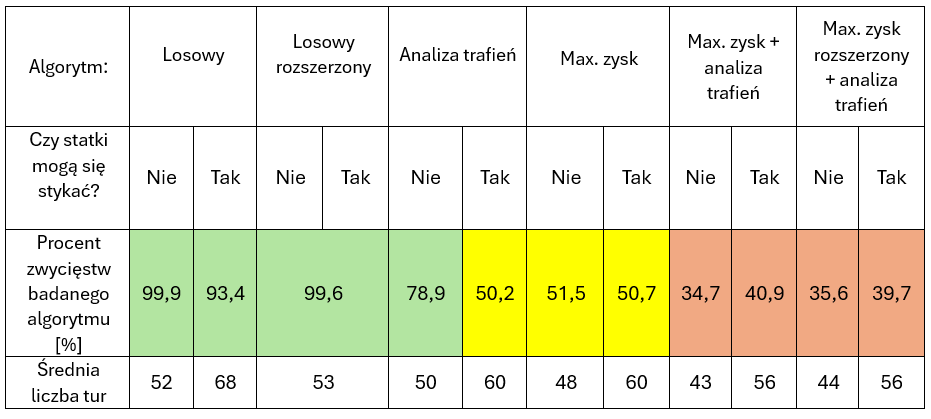
\includegraphics[width=1\linewidth]{img/table-location-heuristic-extended.png}
    \caption{Wyniki testów dla algorytmu opartego na heurystyce maksymalizacji zysku priorytetyzującej dłuższe statki}
\end{table}

\subsubsection{Algorytm oparty na heurystykach maksymalizacji zysku oraz najbardziej prawdopodobnej lokalizacji na podstawie trafień}

Jak widać na tabeli 6.6, algorytm wygrywa w zestawieniu ze wszystkimi pozostałymi algorytmami, poza swoją rozszerzoną wersją. Największy wzrost skuteczności widać przeciwko algorytmom \emph{Analiza trafień} oraz \emph{Max.zysk}. Wynika to z faktu, że badany algorytm jest usprawnieniem \emph{Max.zysk} poprzez umożliwienie algorytmowi 'dobijania' trafionych statków.

\begin{table}[!h]
    \centering
    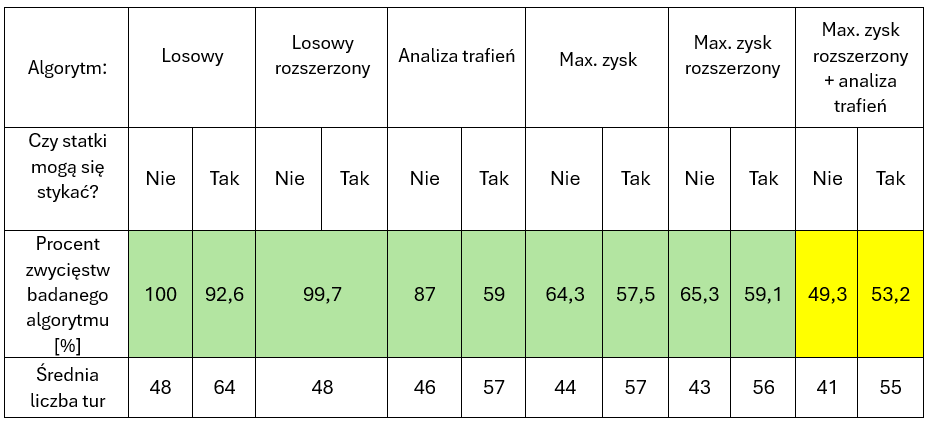
\includegraphics[width=1\linewidth]{img/table-location-hit-heuristic.png}
    \caption{Wyniki testów dla algorytmu opartego na heurystykach maksymalizacji zysku oraz najbardziej prawdopodobnej lokalizacji na podstawie trafień}
\end{table}

\subsubsection{Algorytm oparty na heurystykach maksymalizacji zysku oraz najbardziej prawdopodobnej lokalizacji na podstawie trafień priorytetyzującej dłuższe statki}

Podobnie jak w przypadku 6.2.5, wyniki wersji podstawowej i rozszerzonej algorytmu są bardzo zbliżone. W bezpośrednich starciu wersja rozszerzona jest nieznacznie skuteczniejsza gdy statki nie mogą się ze sobą stykać. W przeciwnym wypadku, lepiej wypada wersja podstawowa algorytmu. W starciach z pozostałymi algorytmami wyniki są zbliżone.

\begin{table}[!h]
    \centering
    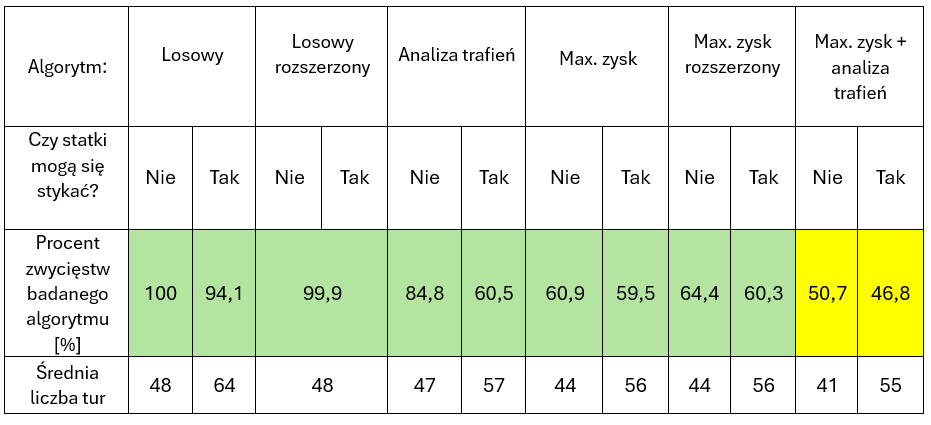
\includegraphics[width=1\linewidth]{img/table-location-extended-hit-heuristic.png}
    \caption{Wyniki testów dla algorytmu opartego na heurystykach maksymalizacji zysku oraz najbardziej prawdopodobnej lokalizacji na podstawie trafień priorytetyzującej dłuższe statki}
\end{table}

\subsection{Podsumowanie}

Aby wyłonić najskuteczniejszy algorytm, stworzone zostały tabele 6.8 oraz 6.9. Przedstawiają one zestawienie pojedynków pomiędzy wszystkimi algorytmami. Tabela 6.8 przedstawia wyniki, gdy statki nie mogą się ze sobą stykać, a tabela 6.9. przeciwny przypadek. W każdej kolumnie na zielono zaznaczone zostały komórki zawierające najwyższą skuteczność. Oznacza to, że algorytm przypisany do danego wiersza, był najskuteczniejszy w starciu z algorytmem przypisanym do danej kolumny.

Korzystając z tych tabelę, można zaobserwować:

\begin{itemize}
    \item Gdy statki nie mogą się ze sobą stykać, podstawowa wersja  \emph{Max. zysk + analiza trafień} jest najskuteczniejsza w prawie wszystkich przypadkach. 
    \item Gdy statki mogą się ze sobą stykać, rozszerzona wersja  \emph{Max. zysk + analiza trafień} jest najskuteczniejsza w prawie wszystkich przypadkach, poza bezpośrednim starciem ze swoją podstawową wersją.
\end{itemize}

Widać więc wyraźnie wpływ różnicy zasad na wyniki. Ciekawe jest to, że w obu przypadkach ogólnie najskuteczniejszy algorytm przegrywał w starciu ze swoim drugim wariantem.

Aby ostatecznie rozstrzygnąć, który algorytm jest skuteczniejszy spróbowano również policzyć ich ogólną skuteczność. Dokonano tego poprzez obliczenie średniej ze skuteczności przeciwko poszczególnym algorytmom. Przekłada się to na następujące wyniki procentowe:

\begin{itemize}
    \item 70,94\% dla wersji podstawowej
    \item 70,51\% dla wersji rozszerzonej
\end{itemize}

Nieznacznie skuteczniejszy jest więc wersja podstawowa \emph{Max. zysk + analiza trafień}.
\begin{table}[!h]
    \centering
    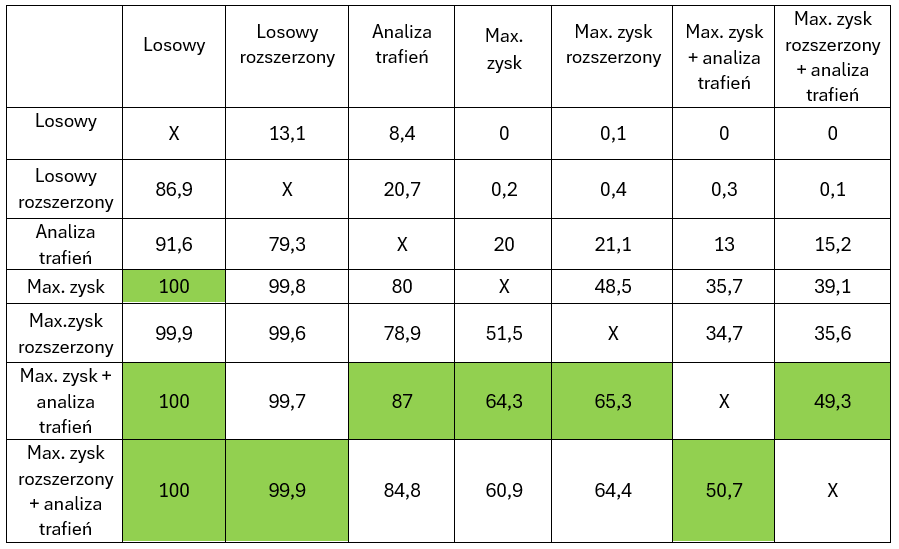
\includegraphics[width=1\linewidth]{img/summary-ships-cant-touch.PNG}
    \caption{Podsumowanie testów gdy statki nie mogą się ze sobą stykać}
\end{table}

\begin{table}[!h]
    \centering
    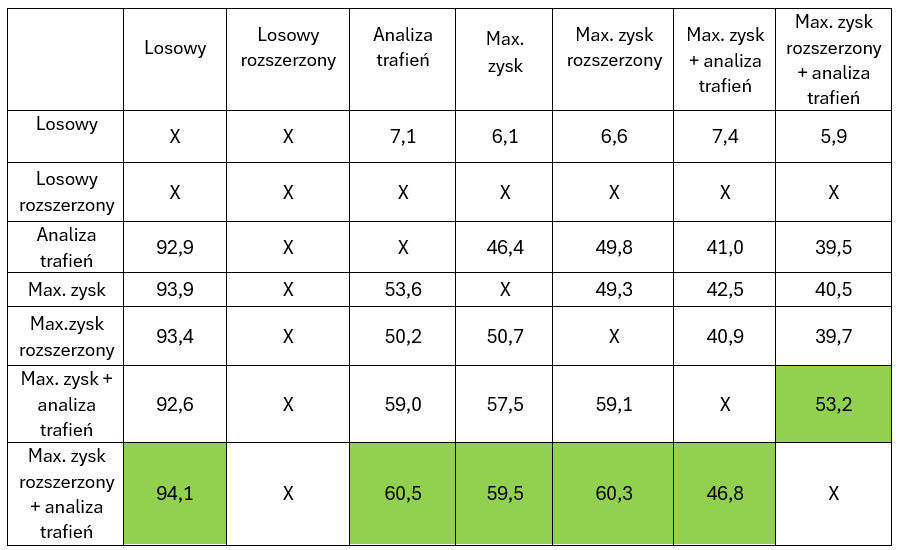
\includegraphics[width=1\linewidth]{img/summary-ships-can-touch.PNG}
    \caption{Podsumowanie testów gdy statki mogą się ze sobą stykać}
\end{table}

Analogicznie obliczono zagregowane skuteczności dla wszystkich algorytmów, co przedstawia tabela 6.10. Przy obliczeniach wykorzystano zapytanie widoczne na listingu 13.

\begin{table}[!h]
    \centering
    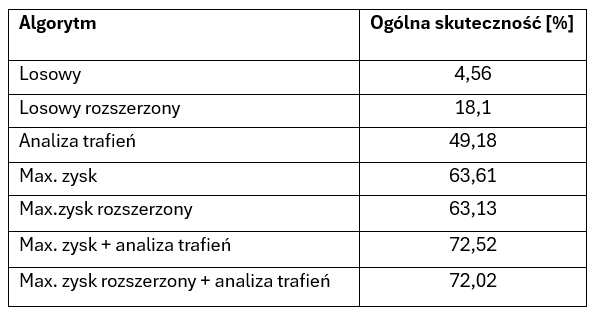
\includegraphics[width=0.7\linewidth]{img/aggregate.PNG}
    \caption{Zagregowane średnie skuteczności poszczególnych algorytmów}
\end{table}

\begin{addmargin}[10mm]{0mm}
\begin{lstlisting}[
    language=SQL,
    numbers=left,
    firstnumber=1,
    caption={Zapytanie do Azure Cosmos DB, w celu uzyskania zagregowanej skuteczności algorytmu},
    aboveskip=0pt
]
SELECT 
    AVG(
        IIF(c.playerMovesCount > c.opponentMovesCount,
        c.playerMovesCount,
        c.opponentMovesCount)
    ) AS avgMaxMoves
FROM c
WHERE (c.playerAiType = {ALG_1} AND c.opponentAiType = {ALG_2}
OR c.playerAiType = {ALG_2} AND c.opponentAiType = {ALG_1})
and c.shipsCanTouch = {WYBRANE_ZASADY}
\end{lstlisting}
\end{addmargin}

Na podstawie wyników stworzono wykres widoczny na rysunku 6.1. Algorytmy zostały posortowane od najmniej do najbardziej skutecznego.

\begin{figure}[!h]
    \label{fig:aggregate-chart}
    \centering 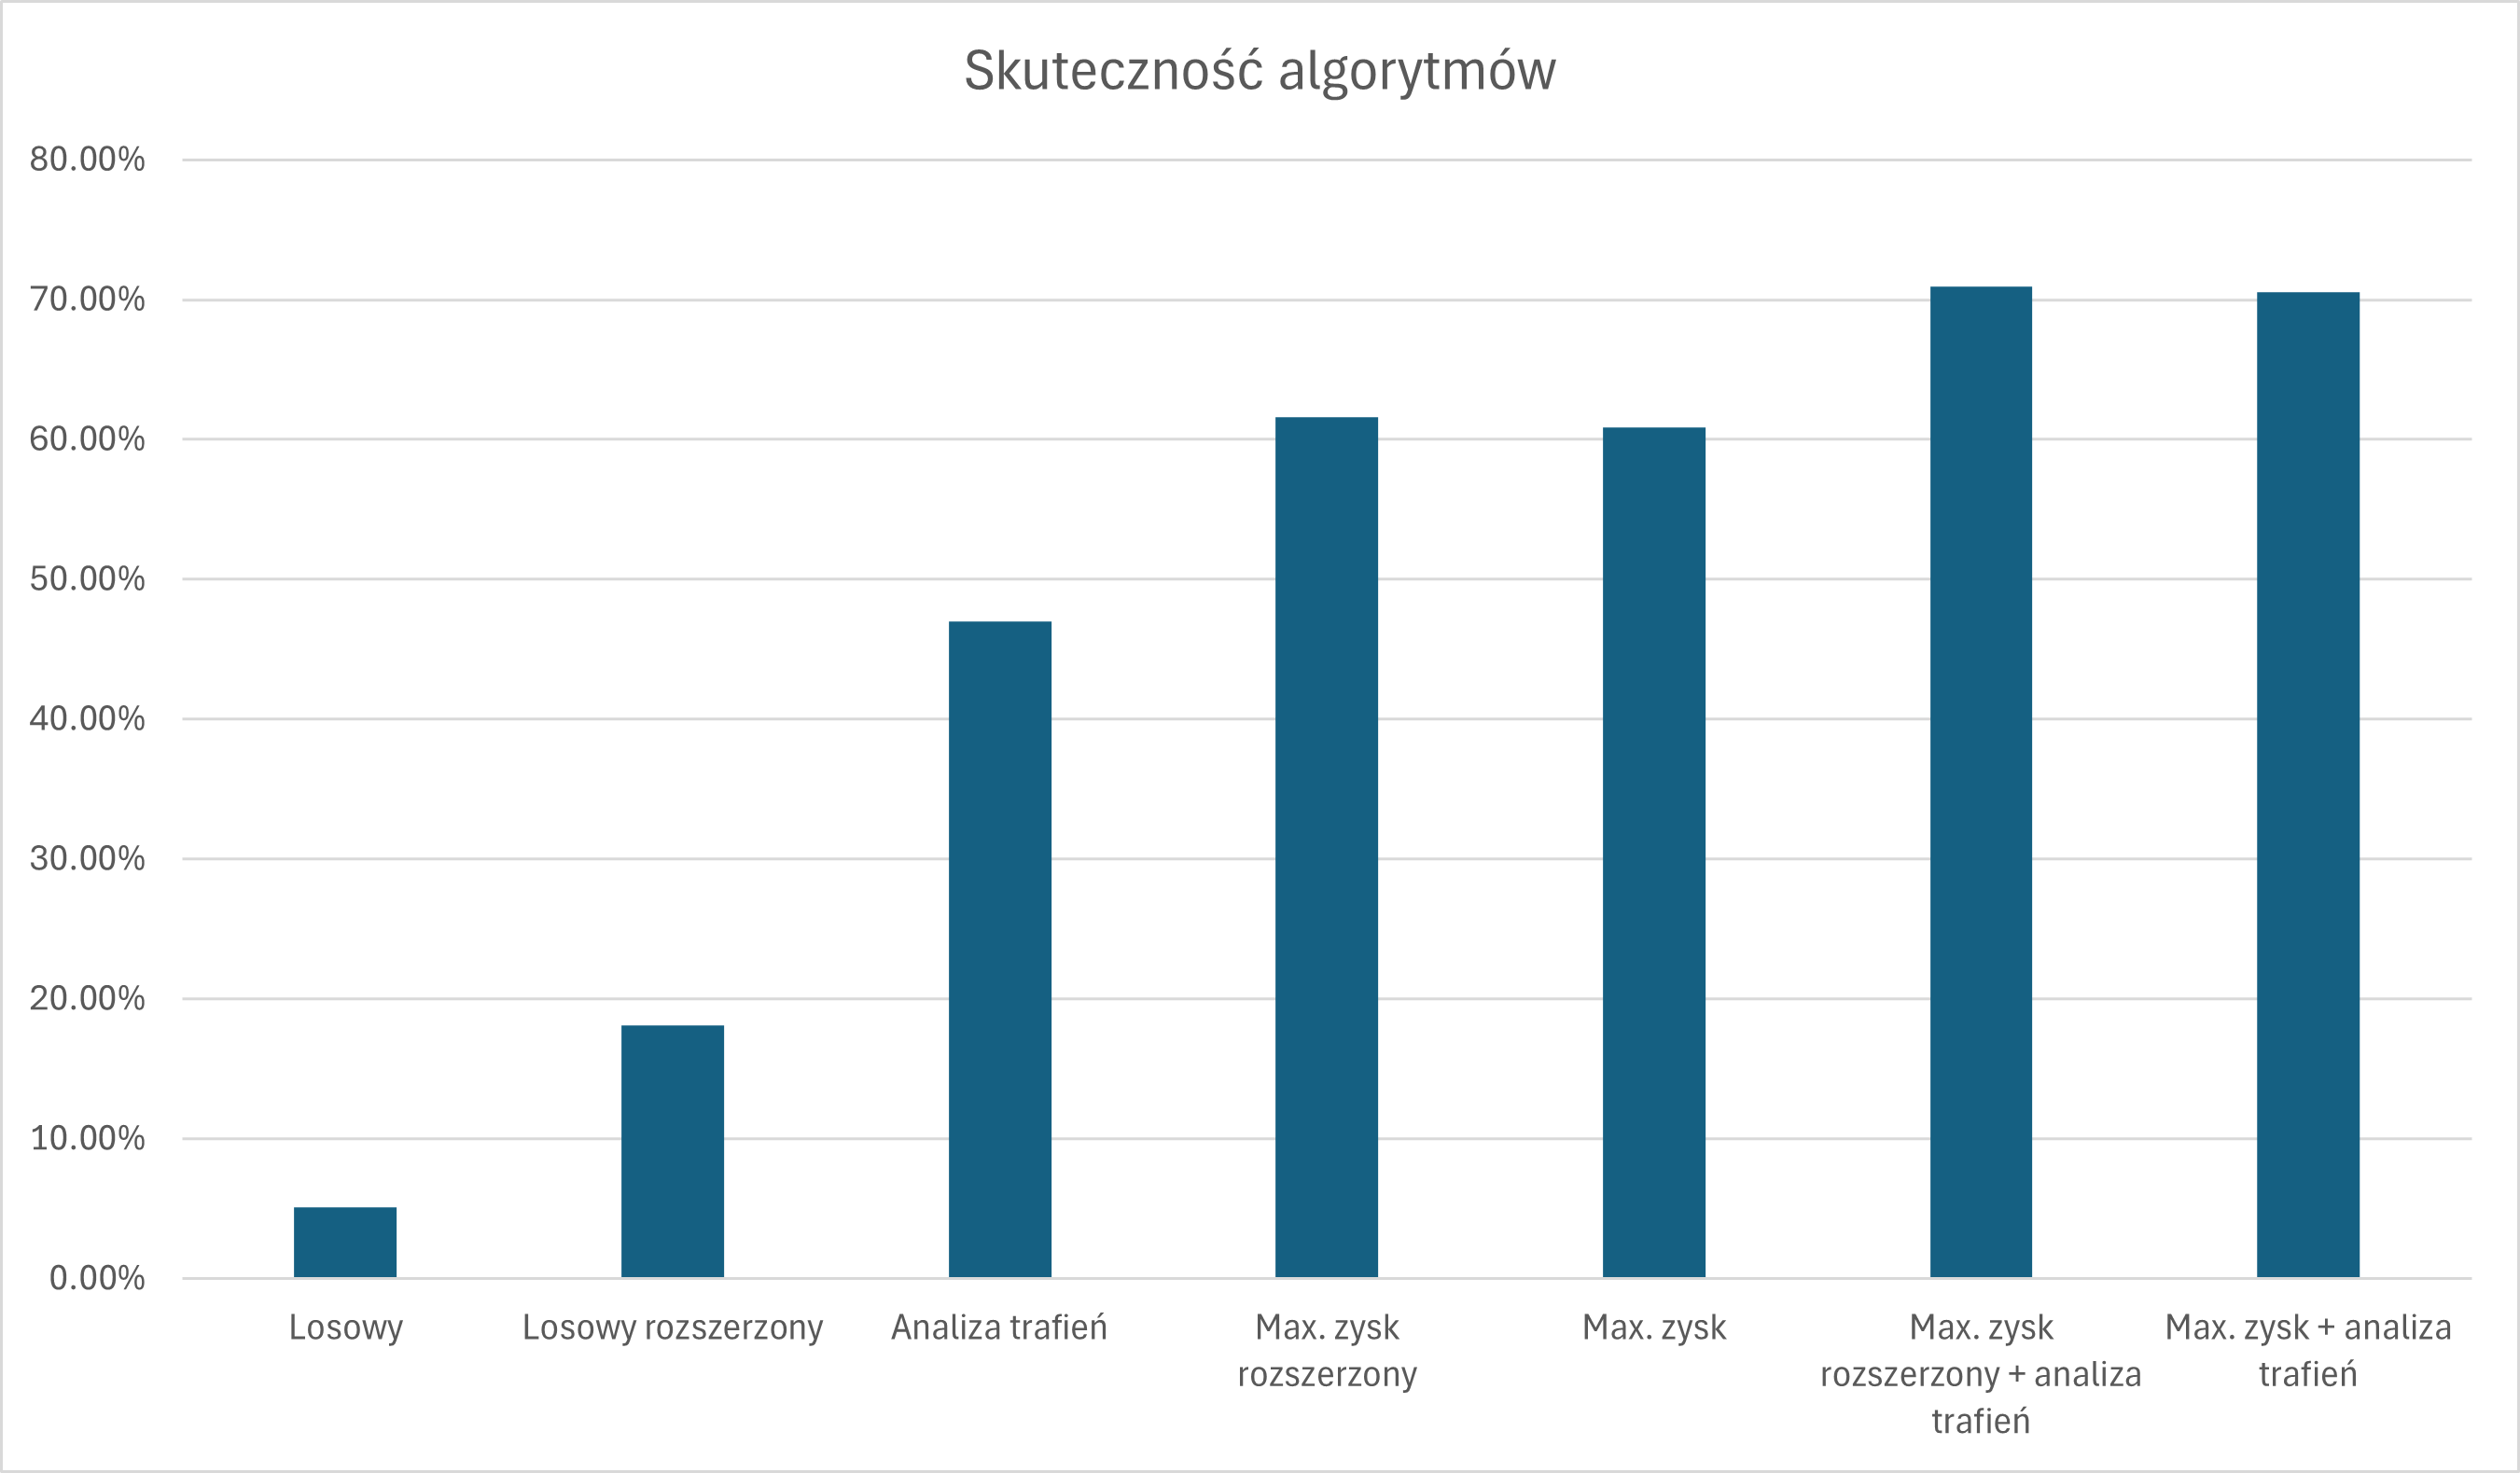
\includegraphics[width=0.9\linewidth]{img/aggregate-chart.png}
    \caption{Wykres zagregowanych średnich dla poszczególnych algorytmów.}
\end{figure}

Utworzono również wykres 6.2 ukazujący skuteczności różnych algorytmów w starciach z algorytmem losowym, aby lepiej zobrazować różnice w skuteczności zależnie od tego czy statki mogą się ze sobą stykać.

\begin{figure}[!h]
    \label{fig:round-avg}
    \centering 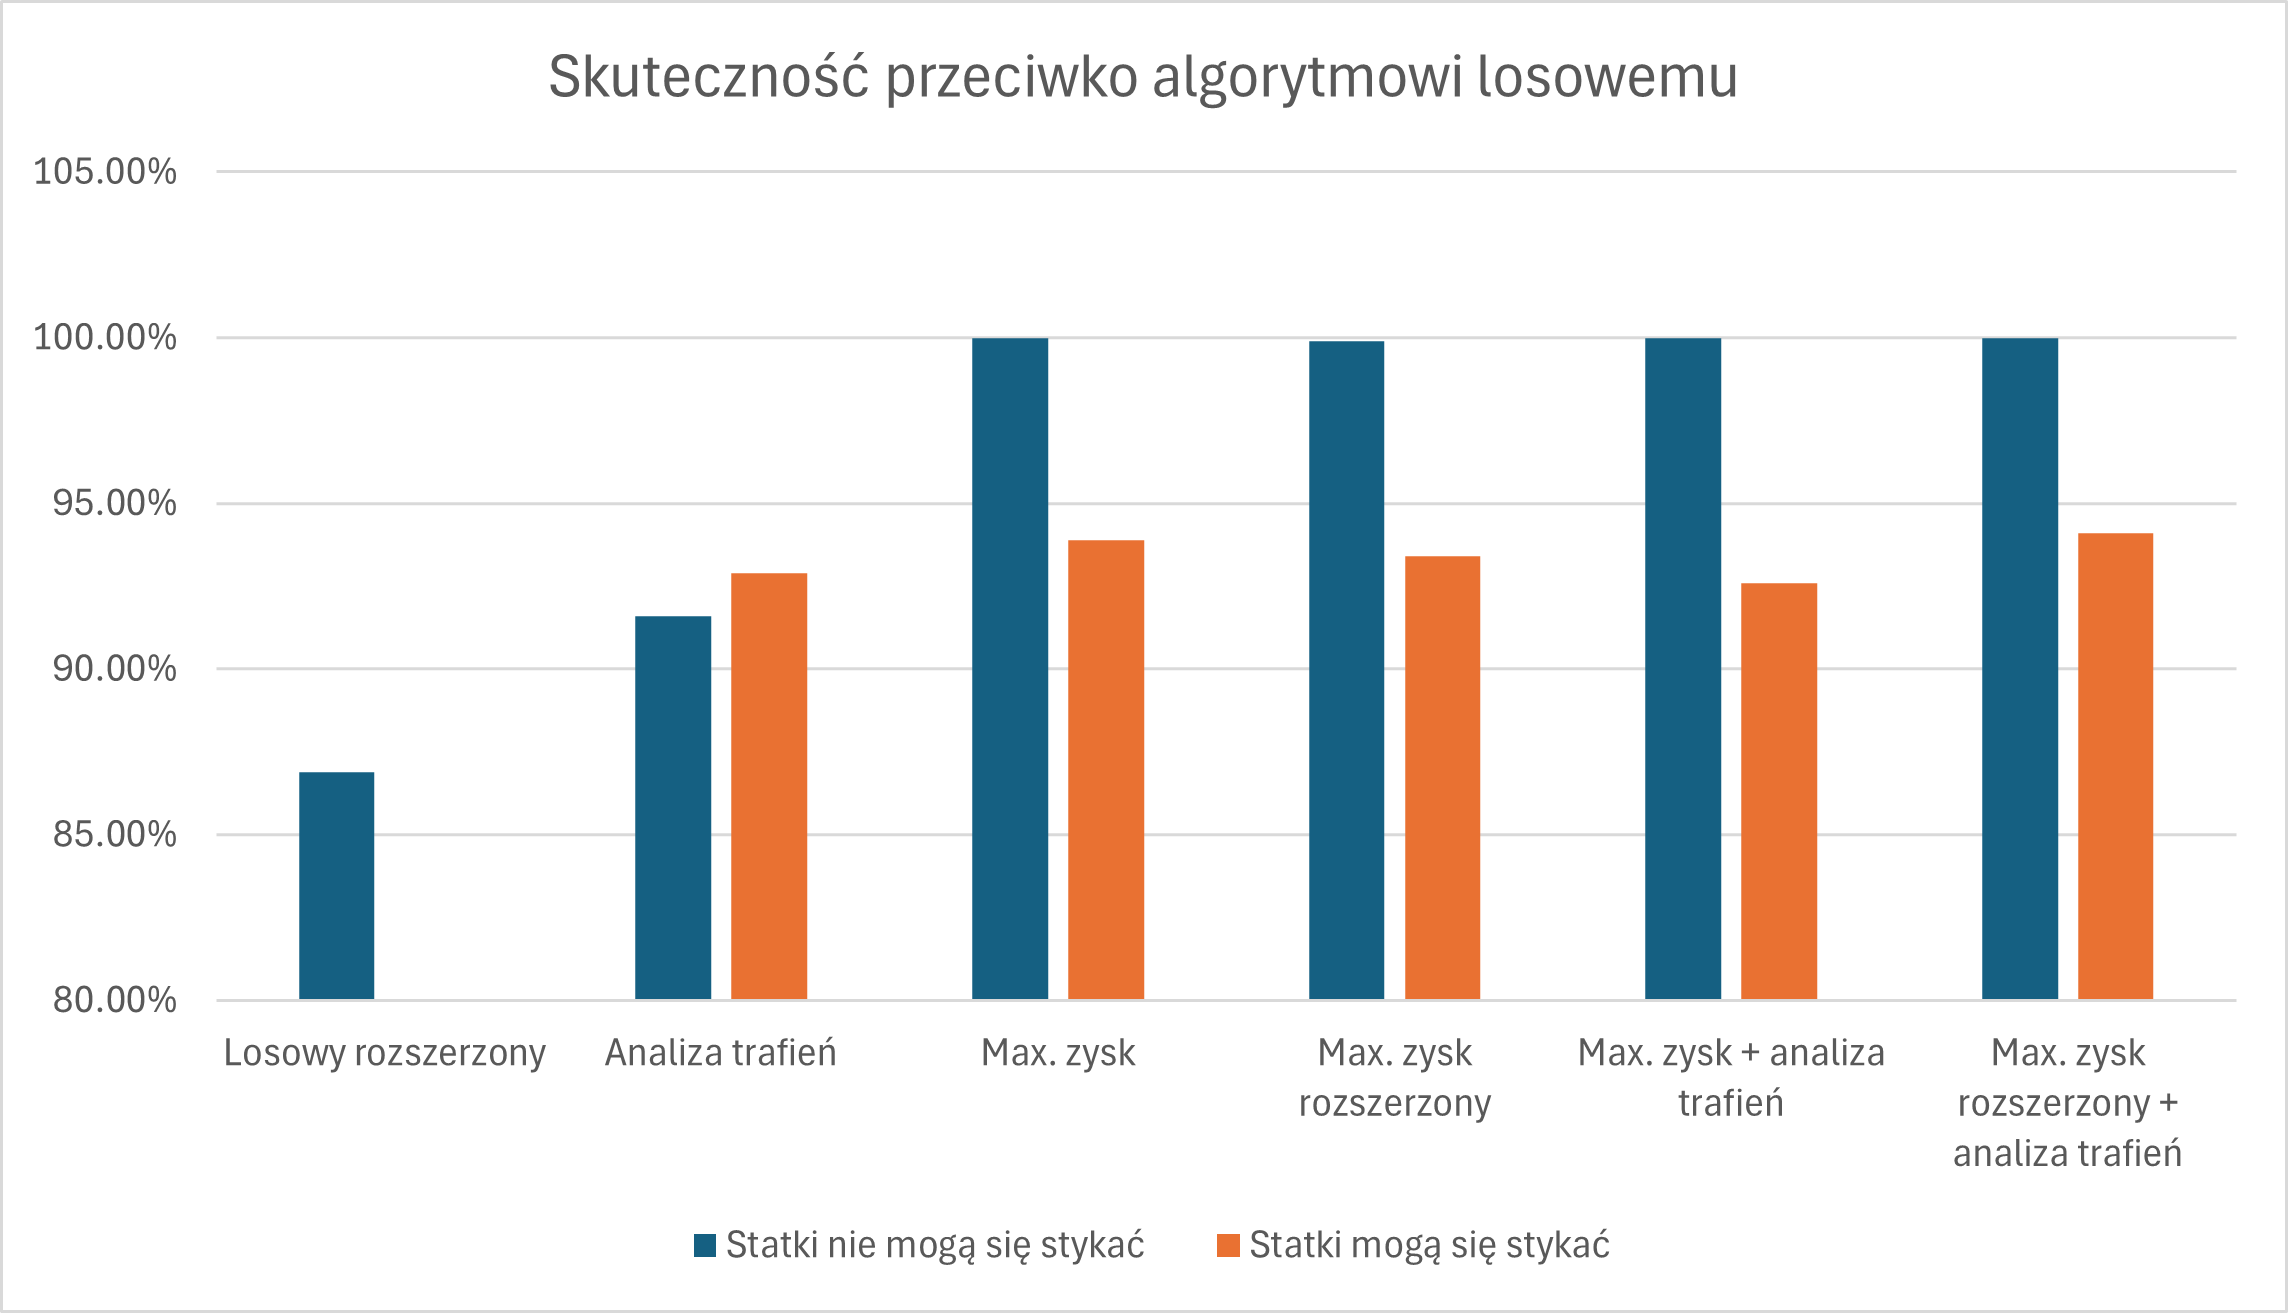
\includegraphics[width=0.9\linewidth]{img/chart-random-scores.png}
    \caption{Skuteczność algorytmów w starciach z algorytmem losowym.}
\end{figure}

Dla wszystkich zestawień algorytmów obliczono również średnią liczbę zagranych tur, zanim jedna ze stron odniosła zwycięstwo. Dane te widoczne są w tabelach 6.1-6.9 oraz na wykresie z rysunku 6.3, gdzie jako punkt odniesienia wykorzystano algorytm losowy.

\begin{figure}[!h]
    \label{fig:round-avg}
    \centering 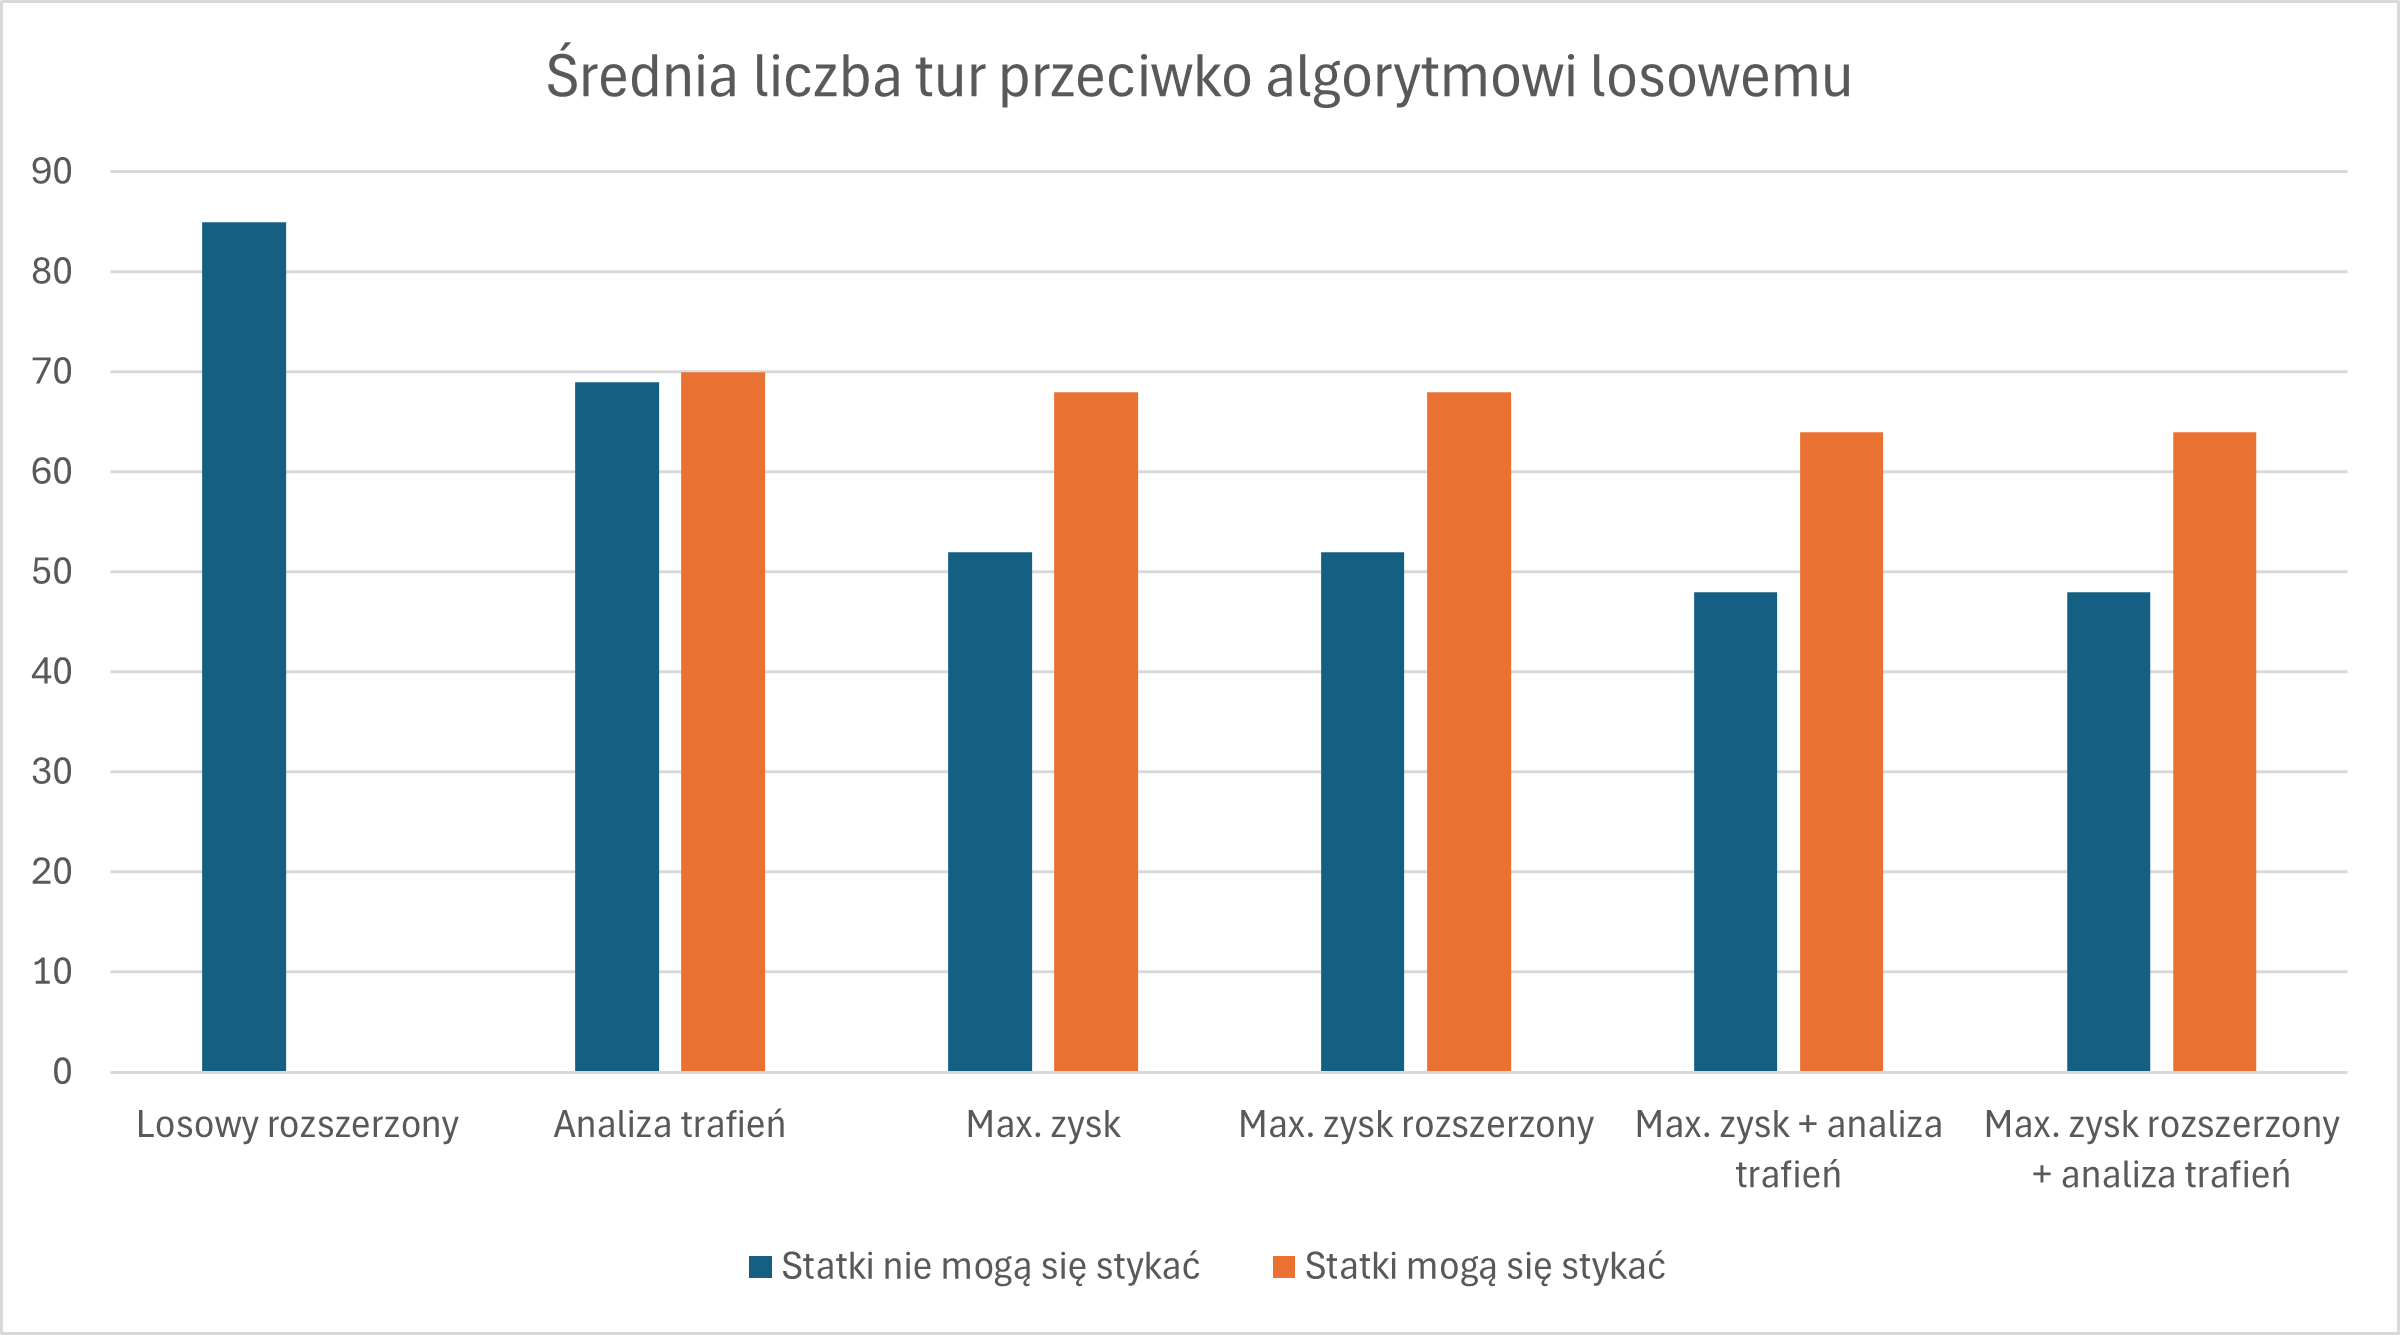
\includegraphics[width=0.9\linewidth]{img/round-count-avg.png}
    \caption{Średnia liczba tur w starciach z algorytmem losowym.}
\end{figure}


\subsection{Analiza rozgrywek z ludźmi}

Niestety nie udało się zebrać wystarczająco dużo danych, aby przeprowadzić dokładną analizę skuteczności algorytmów decyzyjnych przeciwko ludziom. Testy algorytm-algorytm opierały się na 1000 rozgrywek pomiędzy parami algorytmów, dla obu wariantów zasad. W przypadku testów z ludźmi, do analizy potrzebny byłoby 13 000 rozgrywek, ponieważ zaimplementowano 7 algorytmów, w tym jeden który dostępny jest jedynie gdy statki nie mogą się ze sobą stykać. Udało się zebrać dane dotyczące jedynie około 100 rozgrywek, a więc jedynie 1\% potrzebnej liczby. Przeprowadzona na ich podstawie analiza nie jest więc zbyt miarodajna, może być potraktowana raczej jako ciekawostka.

Większość użytkowników preferowała wybór zasad niepozwalających statkom się stykać - dlatego tylko ten przypadek będzie analizowany.

Na tabeli 6.11 oraz obrazującym ją wykresie z rysunku 6.12 widać, że ogólna tendencja skuteczności algorytmów jest podobna. Widać jej stopniowy wzrost, oraz spadek średniej liczby tur potrzebnej do pokonania gracza. Anomalią jest znaczny wzrost skuteczności w przypadku algorytmu \emph{Max. zysk}, ale wynika to najprawdopodobniej z małej próby badawczej. Dodatkowym czynnikiem utrudniającym miarodajną analizę wyników starć algorytm-gracz, jest fakt że nie każdy gracz gra na takim samym poziomie. Teoretycznie słabszy algorytm może mieć zawyżoną skuteczność, jeśli grało z nim  więcej 'słabszych' graczy. Dlatego konieczna jest większa ilość rozgrywek, aby wyeliminować wpływ tych czynników na ogół danych.

\begin{table}[!h]
    \label{fig:vs-people}
    \centering 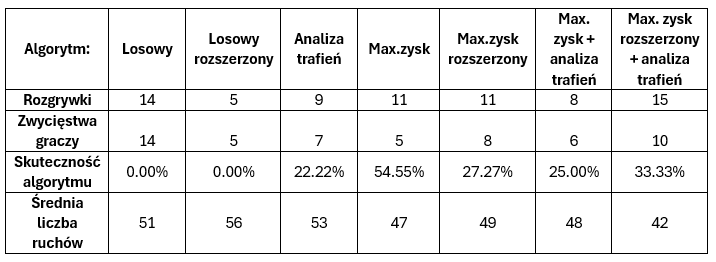
\includegraphics[width=0.9\linewidth]{img/vs_people.PNG}
    \caption{Skuteczność oraz średnia liczba ruchów algorytmów w starciach z graczami.}
\end{table}

\begin{table}[!h]
    \label{fig:vs-people-chart}
    \centering 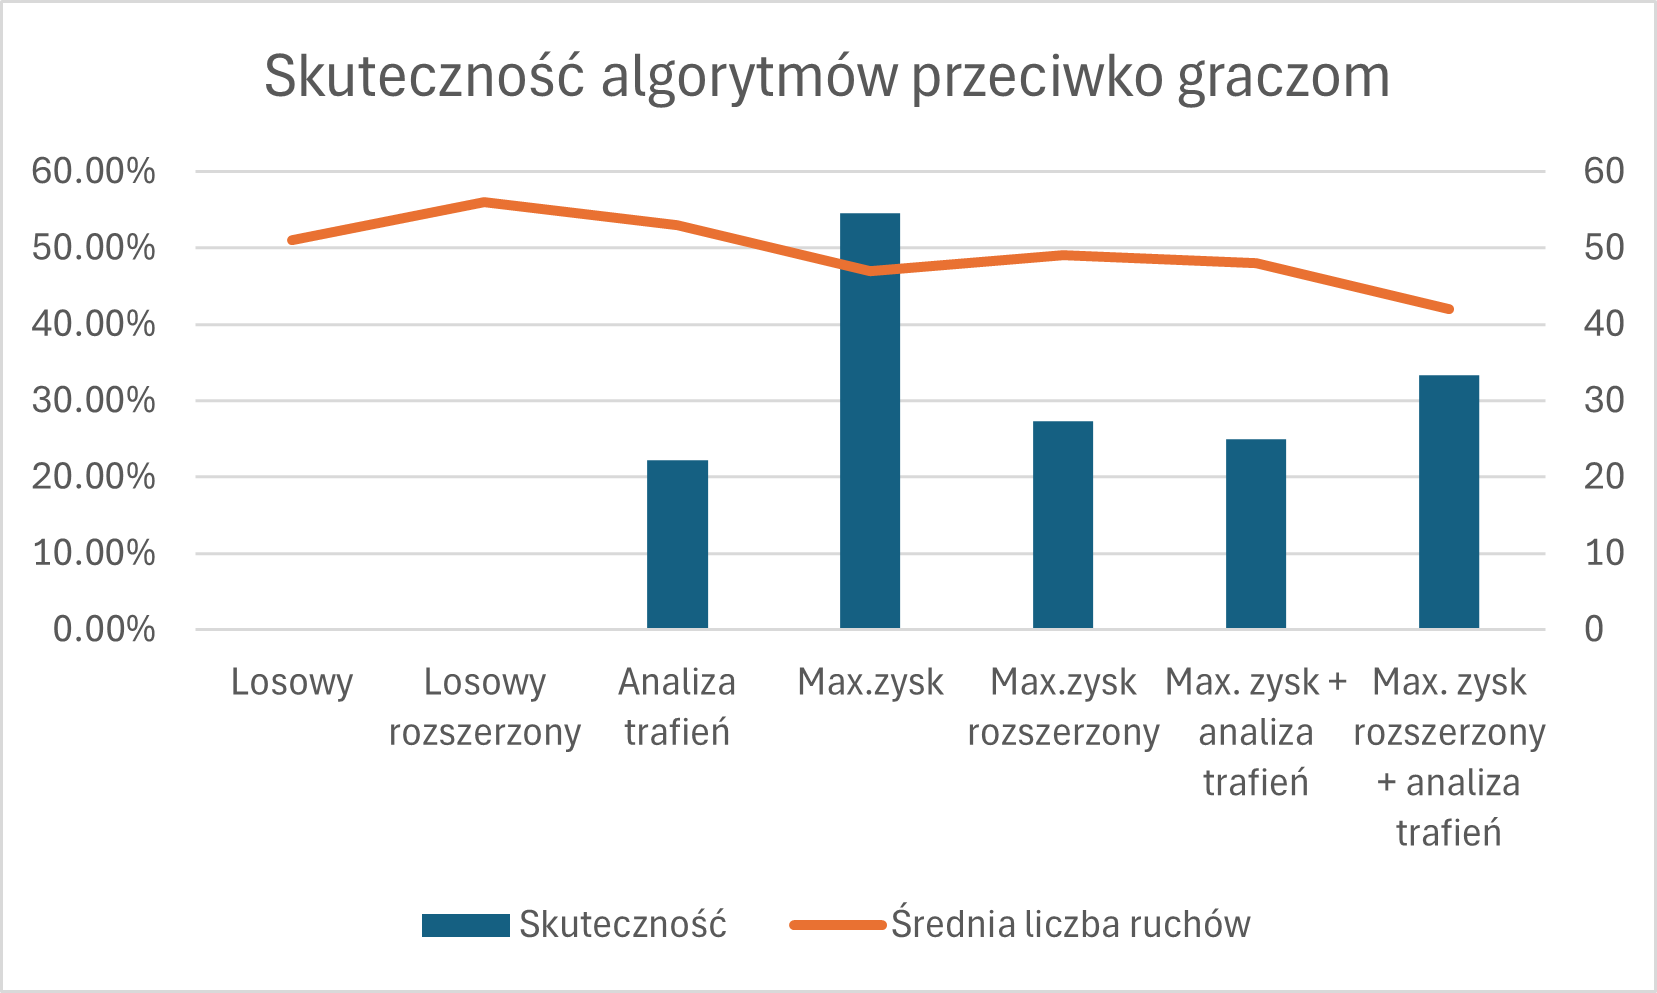
\includegraphics[width=0.9\linewidth]{img/vs_people_chart.png}
    \caption{Wykres przedstawiający skuteczność oraz średnią liczbę ruchów algorytmów w starciach z graczami.}
\end{table}
\newpage % Rozdziały zaczynamy od nowej strony.
\section{Wnioski}

Na podstawie wyników przedstawionych w poprzednim rozdziale, możemy uszeregować algorytmy od najmniej do najbardziej skutecznego:\begin{enumerate}
    \item Algorytm losowy
    \item Rozszerzony algorytm losowy
    \item Algorytm oparty na heurystyce najbardziej prawdopodobnej lokalizacji na podstawie trafień
    \item Algorytm oparty na heurystyce maksymalizacji zysku priorytetyzującej dłuższe statki
    \item Algorytm oparty na heurystyce maksymalizacji zysku ze strzału
        \item Algorytm oparty na heurystykach maksymalizacji zysku oraz najbardziej prawdopodobnej lokalizacji na podstawie trafień priorytetyzującej dłuższe statki
    \item Algorytm oparty na heurystykach maksymalizacji zysku oraz najbardziej prawdopodobnej lokalizacji na podstawie trafień
\end{enumerate}

Na wykresie widocznym na rysunku 6.1. widzimy że pomiędzy heurystyką maksymalizacji zysku ze strzału oraz heurystyką najbardziej prawdopodobnej lokalizacji na podstawie trafień, to ta pierwsza jest bardziej skuteczna. Tak więc minimalizacja możliwych położeń statków na mapie jest bardziej opłacalna, nawet jeśli algorytm nie potrafi analizować trafień w celu 'dobijania' statków. Generalnie, z wykresu wyraźnie widać, że im mniej losowości w algorytmie, tym jest skuteczniejszy - algorytm \emph{Analiza trafień} losowo wybiera ostrzeliwane komórki, jeśli nie ma żadnego trafienia, które może analizować.

Na wykresie widać również brak znaczącej różnicy pomiędzy algorytmami priorytetyzującymi dłuższe statki, a podstawowymi wariantami tychże algorytmów. Jest to prawdopodobnie spowodowane faktem, że trafienie największego statku zazwyczaj nie jest największym wyzwaniem w rozgrywce. Najbardziej problematyczne jest raczej trafienie najmniejszego statku - żadna heurystyka nie jest w stanie pomóc w odnalezieniu jego lokalizacji.

W wynikach widać też, że gdy statki mogą się ze sobą stykać, wyniki starć pomiędzy poszczególnymi algorytmami są bardziej wyrównane. Algorytmy losowe nadal są zdecydowanie najsłabsze, ale algorytmy oparte na heurystykach mają skuteczności w przedziale około 40-60\%. W przypadku tego wariantu zasad, na skuteczności wiele tracą algorytmy oparte na heurystyce maksymalizacji zysku ze strzału. Mniej ograniczeń lokalizacji statku przez zasady, oznacza że istnieje więcej potencjalnych rozmieszczeń statków na planszy przeciwnika. Algorytm potrzebuje więcej ruchów, aby eliminować, te możliwe położenia. 

Tę teorię potwierdza analiza skuteczności wszystkich algorytmów przeciwko algorytmowi losowemu, która jest widoczna na rysunku 6.2. Łatwo zauważyć, że prawie we wszystkich przypadkach, skuteczności  znacznie różnią się zależnie od wybranych zasad. Jedynym wyjątkiem jest algorytm oparty na heurystyce najbardziej prawdopodobnej lokalizacji na podstawie trafień. Algorytm ten wybiera losowo komórki do ostrzału, jeśli na planszy nie ma żadnego trafienia - nie ma więc na niego wpływu fakt, że statki mogą się ze sobą stykać.

Różnicę dobrze widać też na rysunku 6.2, który przedstawia średnią liczbę tur w zależności od tego z jakim algorytmem mierzył się algorytm losowy. W przypadku wszystkich algorytmów poza \emph{Analizą trafień}, liczba tur gdy statki mogą się ze sobą stykać jest znacznie wyższa niż w przeciwnym wypadku. Widać też że liczba tur spada znacznie wolniej wraz ze wzrostem zaawansowania algorytmu. Wynika to z wcześniej wspomnianego faktu, że heurystyka maksymalizacji zysku ze strzału traci na efektywności gdy statki mogą się ze sobą stykać.

W tabelach 6.1-6.9 widać dobrze, że im skuteczniejszy jest dany algorytm, tym krótsze są średnio jego rozgrywki. Średnio najmniej tur potrzebnych było w starciach algorytmów \emph{Max. zysk + analiza trafień} oraz \emph{Max. zysk rozszerzony + analiza trafień}.


\subsection{Ograniczenia pracy}
Nie udało się niestety zebrać wystarczająco dużo danych z rozgrywek człowiek-algorytm, aby ocenić skuteczność algorytmów w starciach z człowiekiem

\newpage % Rozdziały zaczynamy od nowej strony.
\section{Podsumowanie}

W rozdziale 1.3 postawione zostały 3 pytania:

\begin{enumerate}
    \item Który algorytm decyzyjny jest najbardziej skuteczny?
    \item Co ma wpływ na skuteczność algorytmów?
    \item Czy skuteczność algorytmów różni się w zależności od tego czy gra przeciwko człowiekowi, czy innemu algorytmowi?
\end{enumerate}

Na podstawie testów oraz analizy wyników podjęto próbę odpowiedzi na powyższe pytania.

Najbardziej skutecznym algorytmem okazał się algorytm oparty na heurystykach maksymalizacji zysku oraz najbardziej prawdopodobnej lokalizacji na podstawie trafień, aczkolwiek nie miał on zbyt dużej przewagi nad swoją rozszerzoną wersję, priorytetyzującą dłuższe statki.

Największy wpływ na skuteczność algorytmów miała minimalizacji możliwych rozmieszczeń statków, dzięki heurystyce maksymalizacji zysku ze strzału. Strategiczne ostrzeliwanie komórek, na których może leżeć wiele różnych wariantów statków, prowadzi do zawężenia późniejszych rozważań, a co za tym idzie, szybszego (i zwycięskiego) zakończenia rozgrywki.

Niestety, nie udało się zebrać wystarczająco dużo danych, aby przeprowadzić dogłębną analizę skuteczności przeciwko ludziom. Jednak nawet przy małej próbie badawczej widać, że algorytmy oparte na zaimplementowanych heurystykach są znacznie skuteczniejsze od algorytmów losowych. Istnieje duża szansa, że dalsze badania mogłyby dać podobne wyniki do analizy opartej na starciach pomiędzy algorytmami.

\subsection{Przyszłe kierunki badań}

Napisana w ramach pracy magisterskiej aplikacja pozostawia wiele możliwości do dalszego rozwoju i badań:
\begin{itemize}
    \item Dokładniejsza analiza skuteczności przeciwko ludziom. W tym celu należałoby zebrać dużo więcej danych - co najmniej tyle ile w przypadku analizy starć algorytm-algorytm. Potrzebne by było zatem 1000 rozgrywek dla każdego algorytmu, w obu wariantach zasad. Zaimplementowano 7 algorytmów, w tym jeden, który dostępny jest tylko gdy statki nie mogą się ze sobą stykać - ostateczna liczba potrzebna do dokładnej analizy to 13 000 rozgrywek.
    \item Implementacja algorytmów decyzyjnych do rozstawiania statków. W tym celu można by wykorzystać istniejące algorytmy, ale "odwrócić" ich działanie. Nowe algorytmy unikałyby najbardziej prawdopodobnych lokalizacji statków.
    \item Wykorzystanie uczenia maszynowego do implementacji kolejnych algorytmów decyzyjnych przeciwnika. Dane zebrane podczas rozgrywek człowiek-algorytm oraz algorytm-algorytm mogłyby służyć jako zbiór danych treningowych. 
\end{itemize}

\indent\ 

%--------------------------------------------
% Literatura
%--------------------------------------------
\cleardoublepage % Zaczynamy od nieparzystej strony
\printbibliography

%--------------------------------------------
% Spisy (opcjonalne)
%--------------------------------------------
\newpage
\pagestyle{plain}

% Wykaz symboli i skrótów.
% Pamiętaj, żeby posortować symbole alfabetycznie
% we własnym zakresie. Ponieważ mało kto używa takiego wykazu,
% uznałem, że robienie automatycznie sortowanej listy
% na poziomie LaTeXa to za duży overkill.
% Makro \acronymlist generuje właściwy tytuł sekcji,
% w zależności od języka.
% Makro \acronym dodaje skrót/symbol do listy,
% zapewniając podstawowe formatowanie.
% //AB
% \vspace{0.8cm}
% \acronymlist
% \acronym{EiTI}{Wydział Elektroniki i Technik Informacyjnych}
% \acronym{PW}{Politechnika Warszawska}
% \acronym{WEIRD}{ang. \emph{Western, Educated, Industrialized, Rich and Democratic}}

\listoffigurestoc     % Spis rysunków.
\vspace{1cm}          % vertical space
\listoftablestoc      % Spis tabel.
\vspace{1cm}          % vertical space
\listofappendicestoc  % Spis załączników

% \renewcommand{\thesubsection}{\Alph{subsection}}


% Załączniki
\newpage
\inputencoding{utf8}
\appendix{Najważniejsze fragmenty kodu aplikacji}

Obie aplikacje są dostępne w repozytoriach na GitHubie:
\begin{itemize}
    \item Frontend - \url{https://github.com/kalina559/battleships-game}
    \item Backend - \url{https://github.com/kalina559/battleships-backend}
\end{itemize}

Są również dostępne na płytce dołączonej do pracy, spakowane w formacie .

\tocless\subsection{Frontend}

\tocless\subsubsection{App.vue}

W pliku App.vue, widocznym na listingu 14, znajduję się główna część aplikacji. Języki HTML oraz CSS wykorzystane są do zdefiniowania strony wizualnej, JavaScript zaś implementuje logikę. W poniższym 
App.vue wykorzystuje pozostałe komponenty zdefiniowane w projekcie, między innymi Header.vue, UserGrid.vue czy OpponentGrid.vue. Dzięki temu ma dostęp do zdarzeń emitowanych przez te komponenty, takich jak na przykład ustawienie statku, czy wybór komórki na planszy przeciwnika.

\begin{addmargin}[0mm]{0mm}
\begin{lstlisting}[
    language=JavaScript,
    numbers=left,
    firstnumber=0,
    caption={Komponent UserGrid.vue},
    aboveskip=0pt,
    breaklines=true
]
<template>
  <div id="app">
    <Header />
    <div class="content">
      <div class="language-switcher">
        <span @click="changeLanguage('en')" class="fi fi-gb"
        :title="$t('englishLanguage')"></span>
        <span @click="changeLanguage('pl')" class="fi fi-pl"
        :title="$t('polishLanguage')"></span>
      </div>
      <Menu v-if="!gameStarted" @startGame="startGame" />
      <div v-if="gameStarted" class="grids">
        <div class="phase">{{ $t(gamePhaseText) }}</div>
        <OpponentGrid :ships="opponentShips" :showShips=false
        :shots="playerShots" @cellSelected="handleUserShot"
          :disabled="currentPlayer !== user"
          :feedbackMessage=$t(opponentGridFeedbackMessage) />
        <UserGrid :ships="playerShips" :shots="opponentShots"
        @shipPlaced="onShipPlaced"
          :feedbackMessage=$t(playerGridFeedbackMessage)
          :shipsCanTouch="shipsCanTouch" />
      </div>
      <Help />
      <div v-if="winner" class="modal">
        <div class="modal-content">
          <p>{{ $t(winnerMessage) }}</p>
          <button @click="resetGame">{{ $t('playAgain') }}</button>
        </div>
      </div>
    </div>
  </div>
</template>

<script>
import { v4 as uuidv4 } from 'uuid';
import Header from './components/Header.vue';
import UserGrid from './components/UserGrid.vue';
import OpponentGrid from './components/OpponentGrid.vue';
import Help from './components/Help.vue';
import Menu from './components/Menu.vue';
import GameApi from './api/GameApi';

const FEEDBACK_OPPONENT_PLACEHOLDER = 'feedbackOpponentPlaceholder';
const FEEDBACK_PLAYER_PLACEHOLDER = 'feedbackPlayerPlaceholder';
const FEEDBACK_PLAYER_SINK = 'feedbackPlayerSink';
const FEEDBACK_PLAYER_HIT = 'feedbackPlayerHit';
const FEEDBACK_PLAYER_MISS = 'feedbackPlayerMiss';
const FEEDBACK_OPPONENT_SINK = 'feedbackOpponentSink';
const FEEDBACK_OPPONENT_HIT = 'feedbackOpponentHit';
const FEEDBACK_OPPONENT_MISS = 'feedbackOpponentMiss';

const WAITING_FOR_OPPONENT_SHIPS = 'waitingForOpponentToDeployShips';
const WAITING_FOR_PLAYER_SHIPS = 'waitingForUserToDeployShips';
const PLAYER_TURN = 'yourTurn';
const OPPONENT_TURN = 'opponentsTurn';

const GamePhase = Object.freeze({
    WaitingForOpponentShips: 1,
    WaitingForPlayerShips: 2,
    PlayerTurn: 3,
    OpponentTurn: 4
});

const Player = Object.freeze({
    User: 1,
    Opponent: 2
});

export default {
  name: 'App',
  components: {
    Header,
    UserGrid,
    OpponentGrid,
    Help,
    Menu
  },
  data() {
    return {
      gameStarted: false,
      gamePhase: GamePhase.WaitingForPlayerShips,
      playerShips: [],
      opponentShips: [],
      playerShipsSet: false,
      opponentShipsSet: false,
      currentPlayer: null,
      opponentShots: [],
      playerShots: [],
      winner: null,
      opponentGridFeedbackMessage: FEEDBACK_OPPONENT_PLACEHOLDER,
      playerGridFeedbackMessage: FEEDBACK_PLAYER_PLACEHOLDER,
      sessionId: null,
      shipsCanTouch: false,
      user: Player.User
    };
  },
  computed: {
    gamePhaseText() {
      switch (this.gamePhase) {
        case GamePhase.WaitingForPlayerShips:
          return WAITING_FOR_PLAYER_SHIPS;
        case GamePhase.WaitingForOpponentShips:
          return WAITING_FOR_OPPONENT_SHIPS;
        case GamePhase.PlayerTurn:
          return PLAYER_TURN;
        case GamePhase.OpponentTurn:
          return OPPONENT_TURN;
        default:
          return '';
      }
    },
    winnerMessage() {
      return this.winner === Player.User ? 'userWon' : 'aiWon';
    }
  },
  methods: {
    changeLanguage(lang) {
      this.$i18n.locale = lang;
    },
    generateOrRetrieveSessionId() {
      let sessionId = this.getCookie('sessionId');
      if (!sessionId) {
        sessionId = uuidv4();
        this.setCookie('sessionId', sessionId, 365);
        // Set cookie to expire in 1 year
      }
      this.sessionId = sessionId;
      GameApi.setSessionId(this.sessionId);
      // Set the session ID in the API client
    },
    getCookie(name) {
      const value = `; ${document.cookie}`;
      const parts = value.split(`; ${name}=`);
      if (parts.length === 2) return parts.pop().split(';').shift();
    },
    setCookie(name, value, days) {
      const expires =
        new Date(Date.now() + days * 864e5).toUTCString();
      document.cookie =
        `${name}=${value}; expires=${expires}; path=/`;
    },
    async startGame(shipsCanTouch) {
      this.gameStarted = true;
      try {
        this.opponentShips = await GameApi.getOpponentShips();
        this.opponentShipsSet = true;
        this.shipsCanTouch = shipsCanTouch
        this.checkPhaseTransition();
      } catch (error) {
        console.error('Failed to get opponent ships:', error);
      }
    },
    async onShipPlaced(ships) {
      this.playerShips = ships;
      this.playerShipsSet = this.playerShips.length === 5;

      if (this.playerShipsSet) {
        try {
          await GameApi.setUserShips(ships);
          this.checkPhaseTransition();
        } catch (error) {
          console.error('Failed to set user ships:', error);
        }
      } else {
        this.checkPhaseTransition();
      }
    },
    checkPhaseTransition() {
      if (this.playerShipsSet && this.opponentShipsSet) {
        this.determineStartingPlayer();
      } else if (this.playerShipsSet) {
        this.gamePhase = GamePhase.WaitingForOpponentShips;
      } else if (this.opponentShipsSet) {
        this.gamePhase = GamePhase.WaitingForPlayerShips;
      }
    },
    determineStartingPlayer() {
      const randomStart = Math.random() < 0.5;
      this.currentPlayer = randomStart 
        ? Player.User 
        : Player.Opponent;
      this.gamePhase = randomStart 
        ? GamePhase.PlayerTurn
        : GamePhase.OpponentTurn;
      if (!randomStart) {
        this.opponentMove();
      }
    },
    async opponentMove() {
      if (this.currentPlayer !== Player.Opponent) return;
      try {
        const move = await GameApi.opponentShot();
        await this.updateGameState();
        this.playerGridFeedbackMessage = move.isHit 
            ? (move.isSunk ? FEEDBACK_OPPONENT_SINK
            : FEEDBACK_OPPONENT_HIT) : FEEDBACK_OPPONENT_MISS;

        this.checkIfWinner(move, Player.Opponent);
      } catch (error) {
        console.error('Failed to get opponent move:', error);
      }
    },
    async handleUserShot(x, y) {
      if (this.currentPlayer !== Player.User) return;
      try {
        const move = await GameApi.userShot({ x, y });
        await this.updateGameState();
        this.opponentGridFeedbackMessage = move.isHit
            ? (move.isSunk ? FEEDBACK_PLAYER_SINK
            : FEEDBACK_PLAYER_HIT) : FEEDBACK_PLAYER_MISS;

        this.checkIfWinner(move, Player.User);
      } catch (error) {
        console.error('Failed to handle user shot:', error);
      }
    },
    async checkIfWinner(move, side) {
      if(move.win == true){
          this.winner = side;
        } else {
          this.switchTurn();
        }
    },
    async updateGameState() {
      try {
        const gameState = await GameApi.getGameState();

        this.playerShips
            .splice(0, this.playerShips.length,
                ...gameState.userShips);
        this.opponentShips
            .splice(0, this.opponentShips.length,
                ...gameState.opponentShips);
        this.playerShots
            .splice(0, this.playerShots.length,
                ...gameState.playerShots);
        this.opponentShots
            .splice(0, this.opponentShots.length,
                ...gameState.opponentShots);
        this.shipsCanTouch = gameState.shipsCanTouch;

      } catch (error) {
        console.error('Failed to update game state:', error);
      }
    },
    switchTurn() {
      this.currentPlayer = this.currentPlayer === Player.User
        ? Player.Opponent
        : Player.User;
      this.gamePhase = this.currentPlayer === Player.User
        ? GamePhase.PlayerTurn
        : GamePhase.OpponentTurn;
      if (this.currentPlayer === Player.Opponent) {
        setTimeout(() => {
          this.opponentMove();
        }, 1000);
      }
    },
    resetGame() {
      this.gameStarted = false;
      this.gamePhase = GamePhase.WaitingForPlayerShips;
      this.playerShips = [];
      this.opponentShips = [];
      this.playerShipsSet = false;
      this.opponentShipsSet = false;
      this.currentPlayer = null;
      this.opponentShots = [];
      this.playerShots = [];
      this.winner = null;
      this.opponentGridFeedbackMessage = '';
      this.playerGridFeedbackMessage = '';
    }
  },
  mounted() {
    this.generateOrRetrieveSessionId();
  }
};
</script>

<style>
.content {
  display: flex;
  flex-direction: column;
  align-items: center;
}

.language-switcher {
  display: flex;
  justify-content: center;
  margin-bottom: 10px;
}

.language-switcher img {
  cursor: pointer;
  margin: 0 10px;
}

.grids {
  display: flex;
  flex-direction: column;
  align-items: center;
}

.phase {
  margin-bottom: 20px;
  font-size: 18px;
  font-weight: bold;
}

.modal {
  position: fixed;
  top: 50%;
  left: 50%;
  transform: translate(-50%, -50%);
  background-color: white;
  padding: 20px;
  border: 1px solid #333;
  box-shadow: 0 0 10px rgba(0, 0, 0, 0.5);
  z-index: 1000;
}

.modal-content {
  text-align: center;
}

.language-switcher .fi {
  margin-right: 8px; /* Add spacing between the span elements */
  width: 32px;
  height: 32px;
  cursor: pointer;
}

.language-switcher .fi:last-child {
  margin-right: 0; /* Remove right margin for the last element */
}
</style>

\end{lstlisting}
\end{addmargin}

\tocless\subsubsection{UserGrid.vue}
Komponent UserGrid.vue jest drugim najbardziej złożonym elementem aplikacji frontend. Wynika to z faktu, że konieczne było zaimplementowanie w nim logiki związanej z rozstawianiem statków na planszy gracza. Znajdują się tutaj metody takie jak isOccupied, isAdjacentOccupied, które sprawdzają czy dana pozycja statku jest możliwa do zrealizowania. Użytkownik dostaje informację zwrotną poprzez zmianę koloru statku na kolor zielony lub czerwony. Kolor zielony oznacza, że statek może być postawiony na danej pozycji.

Kontrolowanie zasad byłoby również możliwe poprzez backend, ale uznano że jest to bardzo nieoptymalne rozwiązanie - w trakcie rozstawiania statków gracz może sprawdzać dziesiątki różnych pozycji zanim podejmie swoją decyzję. Odpytywanie tyle razy backendu niepotrzebnie by obciążało aplikację.


\begin{addmargin}[0mm]{0mm}
\begin{lstlisting}[
    language=JavaScript,
    numbers=left,
    firstnumber=0,
    caption={Główny komponent aplikacji App.vue},
    aboveskip=0pt,
    breaklines=true
]
<template>
  <div class="grid">
    <h2>{{ $t('playersGrid') }}</h2>
    <div class="feedback" 
        v-if="feedbackMessage">{{ feedbackMessage }}</div>
    <div class="grid-container" @keydown="handleKeydown"
        tabindex="0" ref="gridContainer">
      <div class="row">
        <div class="corner"></div>
        <div v-for="label in columnLabels" :key="label"
            class="column-label">{{ label }}</div>
      </div>
      <div v-for="(row, rowIndex) in rows" :key="rowIndex" 
        class="row">
        <div class="row-label">{{ rowLabels[rowIndex] }}</div>
        <div v-for="cell in row" :key="cell.id" 
            :class="['cell', getCellClass(rowIndex, cell.id)]">
          <span v-if="isMissCell(rowIndex, cell.id)"
            class="miss-marker">X</span>
        </div>
      </div>
    </div>
    <div class="controls">
      <div class="control-row">
        <button @click="handleKeydown({ key: 'ArrowUp' })">
            ↑
        </button>
      </div>
      <div class="control-row">
        <button @click="handleKeydown({ key: 'ArrowLeft' })">
            ←
        </button>
        <button @click="handleKeydown({ key: 'ArrowDown' })">
            ↓
        </button>
        <button @click="handleKeydown({ key: 'ArrowRight' })">
            →
        </button>
      </div>
      <div class="control-row">
        <button @click="handleKeydown({ key: 'r' })">
        {{ $t('rotateButton') }}
        </button>
            <button @click="handleKeydown({ key: 'Enter' })">
        {{ $t('deployButton') }}
        </button>
      </div>
    </div>
  </div>
</template>


<script>
export default {
  name: 'UserGrid',
  props: {
    ships: {
      type: Array,
      default: () => []
    },
    shots: {
      type: Array,
      default: () => []
    },
    feedbackMessage: {
      type: String,
      default: ''
    },
    shipsCanTouch: {
      type: Boolean,
      default: false
    },
  },
  data() {
    return {
      // eslint-disable-next-line no-unused-vars
      rows: Array.from({ length: 10 }, (_, rowIndex) =>
        Array.from({ length: 10 }, (__, cellIndex) => ({
          id: cellIndex,
          label: ''
        }))
      ),
      rowLabels: 'ABCDEFGHIJ'.split(''),
      columnLabels: Array.from({ length: 10 }, (_, i) => i + 1),
      placedShips: [],
      currentShip: { size: 5, coordinates: [] },
      currentShipDirection: 'horizontal',
      currentShipPosition: { x: 5, y: 5 }
    };
  },
  mounted() {
    this.initCurrentShip();
    window.addEventListener('keydown', this.handleKeydown);
  },
  beforeUnmount() {
    window.removeEventListener('keydown', this.handleKeydown);
  },
  methods: {
    initCurrentShip() {
      this.updateCurrentShipCoordinates();
    },
    handleKeydown(event) {
      if (this.currentShip.size === 0) return;
      const key = event.key;
      switch (key) {
        case 'ArrowUp':
          this.moveShip(-1, 0);
          break;
        case 'ArrowDown':
          this.moveShip(1, 0);
          break;
        case 'ArrowLeft':
          this.moveShip(0, -1);
          break;
        case 'ArrowRight':
          this.moveShip(0, 1);
          break;
        case 'r':
        case 'R':
          this.rotateShip();
          break;
        case 'Enter':
          this.placeShip();
          break;
      }
    },
    moveShip(dx, dy) {
      const newPosition = { x: this.currentShipPosition.x + dx,
        y: this.currentShipPosition.y + dy };
      this.currentShipPosition = newPosition;
      this.updateCurrentShipCoordinates();
    },
    rotateShip() {
      const newDirection =
        this.currentShipDirection === 'horizontal'
            ? 'vertical'
            : 'horizontal';
      this.currentShipDirection = newDirection;
      this.updateCurrentShipCoordinates();
    },
    isValidPosition(position, size, direction) {
      for (let i = 0; i < size; i++) {
        const x = direction === 'horizontal'
            ? position.x
            : position.x + i;
        const y = direction === 'horizontal'
            ? position.y + i 
            : position.y;

        if (x < 0 || x >= 10 || y < 0 || y >= 10 
            || this.isOccupied(x, y)
            || ( !this.shipsCanTouch
                && this.isAdjacentOccupied(x, y))) {
          return false;
        }
      }
      return true;
    },
    isOccupied(x, y) {
      return this.placedShips.some(ship =>
        ship.coordinates.some(coord => coord.x === x && coord.y === y)
      );
    },
    isAdjacentOccupied(x, y) {
      const adjacentOffsets = [
        { dx: -1, dy: -1 }, { dx: -1, dy: 0 }, { dx: -1, dy: 1 },
        { dx: 0, dy: -1 }, { dx: 0, dy: 1 },
        { dx: 1, dy: -1 }, { dx: 1, dy: 0 }, { dx: 1, dy: 1 }
      ];

      return adjacentOffsets.some(offset => {
        const adjacentX = x + offset.dx;
        const adjacentY = y + offset.dy;
        return (
          adjacentX >= 0 && adjacentX < 10 &&
          adjacentY >= 0 && adjacentY < 10 &&
          this.isOccupied(adjacentX, adjacentY)
        );
      });
    },
    updateCurrentShipCoordinates() {
      this.currentShip.coordinates =
        Array.from({ length: this.currentShip.size }, (_, i) => {
        return this.currentShipDirection === 'horizontal'
          ? { x: this.currentShipPosition.x,
            y: this.currentShipPosition.y + i }
          : { x: this.currentShipPosition.x + i,
            y: this.currentShipPosition.y };
      });
    },
    placeShip() {
      if (this.isValidPosition(this.currentShipPosition,
        this.currentShip.size,
        this.currentShipDirection)) {
        this.placedShips.push({ ...this.currentShip });
        this.$emit('shipPlaced', this.placedShips,
            this.currentShip.size);
        this.updateNextShip();
      }
    },
    updateNextShip() {
      if (this.currentShip.size > 1) {
        this.currentShip.size--;
      } else {
        this.currentShip = { size: 0, coordinates: [] };
        // No more ships to place
      }
      this.currentShipPosition = { x: 5, y: 5 };
      // Reset to middle
      this.updateCurrentShipCoordinates();
    },
    getCellClass(rowIndex, cellIndex) {
      if (this.isShotCell(rowIndex, cellIndex)) {
        return this.isHitCell(rowIndex, cellIndex)
            ? 'hit-cell'
            : 'miss-cell';
      }
      if (this.isShipCell(rowIndex, cellIndex)) {
        return 'ship-cell';
      }
      if (this.isCurrentShipCell(rowIndex, cellIndex)) {
        return this.isValidPosition(this.currentShipPosition,
            this.currentShip.size,
            this.currentShipDirection)
                ? 'valid-ship'
                : 'invalid-ship';
      }
      return '';
    },
    isShotCell(rowIndex, cellIndex) {
      return this.shots.some(shot => shot.x === rowIndex
        && shot.y === cellIndex);
    },
    isHitCell(rowIndex, cellIndex) {
      return this.shots.some(shot => shot.x === rowIndex
        && shot.y === cellIndex && shot.isHit);
    },
    isMissCell(rowIndex, cellIndex) {
      const shot = this.shots.find(shot => shot.x === rowIndex
        && shot.y === cellIndex);
      return shot && !shot.isHit;
    },
    isShipCell(rowIndex, cellIndex) {
      return this.placedShips.some(ship =>
        ship.coordinates.some(coord => coord.x === rowIndex
            && coord.y === cellIndex)
      );
    },
    isCurrentShipCell(rowIndex, cellIndex) {
      return this.currentShip.coordinates
        .some(coord => coord.x === rowIndex
        && coord.y === cellIndex);
    }
  }
};
</script>


<style scoped>
.grid {
  display: flex;
  flex-direction: column;
  align-items: center;
}

.feedback {
  font-size: 18px;
  font-weight: bold;
  margin-bottom: 10px;
}

.grid-container {
  display: grid;
  grid-template-columns: 30px repeat(10, 30px);
  grid-template-rows: 30px repeat(10, 30px);
  gap: 2px;
}

.grid-container:focus {
  outline: none;
}

.row {
  display: contents;
}

.cell,
.column-label,
.row-label {
  width: 30px;
  height: 30px;
  display: flex;
  align-items: center;
  justify-content: center;
}

.cell {
  background-color: lightblue;
  border: 1px solid #333;
}

.valid-ship {
  background-color: lightgreen;
}

.invalid-ship {
  background-color: lightcoral;
}

.hit-cell {
  background-color: red;
}

.miss-cell {
  background-color: white;
  position: relative;
}

.miss-marker {
  color: black;
  font-size: 24px;
  position: absolute;
}

.ship-cell {
  background-color: darkblue;
}

.column-label,
.row-label {
  background-color: #f0f0f0;
  font-weight: bold;
}

.corner {
  background-color: #f0f0f0;
}

.controls {
  display: flex;
  flex-direction: column;
  align-items: center;
  margin-top: 20px;
}

.control-row {
  display: flex;
  justify-content: center;
  margin: 5px 0;
}

.controls button {
  margin: 0 5px;
  padding: 10px 20px;
  font-size: 16px;
}
</style>
\end{lstlisting}
\end{addmargin}


\tocless\subsubsection{GameApi}
Plik GameApi.js zawiera definicje metod wykorzystywanych do odpytywania aplikacji backend poprzez zapytania AJAX. W tym celu wykorzystano klienta Axios. Do każdego zapytania dołączany jest header "X-Session-Id", który potrzebny jest do identyfikacji danej sesji gry.

\begin{addmargin}[0mm]{0mm}
\begin{lstlisting}[
    language={JavaScript},
    numbers=left,
    firstnumber=5,
    caption={Plik GameApi.js},
    aboveskip=0pt
]
import axios from 'axios';

const apiClient = axios.create({
  baseURL: process.env.VUE_APP_API_URL,
  withCredentials: true,
  // Include credentials (cookies) with requests
  headers: {
    'Content-Type': 'application/json'
  }
});

let sessionId = null;

function setSessionId(id) {
  sessionId = id;
}

apiClient.interceptors.request.use(config => {
  if (sessionId) {
    config.headers['X-Session-Id'] = sessionId;
  }
  return config;
});

export default {
  setSessionId,
  async getAiTypes(shipsCanTouch) {
    const response = await apiClient.post('/AiType/list',
        shipsCanTouch);
    return response.data;
  },
  async selectAiType(type) {
    await apiClient.post('/AiType/select', type);
  },
  async updateRules(shipsCanTouch) {
    await apiClient.post('/Rules/update', shipsCanTouch);
  },
  async getOpponentShips() {
    const response = await apiClient.get('/ShipLocations/opponent');
    return response.data;
  },
  async setUserShips(shipData) {
    await apiClient.post('/ShipLocations/user', shipData);
  },
  async userShot(position) {
    const response = await apiClient.post('shot/user', position);
    return response.data;
  },
  async opponentShot() {
    const response = await apiClient.get('shot/opponent');
    return response.data;
  },
  async getGameState() {
    const response = await apiClient.get('gamestate/get');
    return response.data;
  },
  async clearGameState() {
    await apiClient.get('gamestate/clear');
  }
};

\end{lstlisting}
\end{addmargin}

\tocless\subsection{Backend}

\tocless\subsubsection{Program.cs}

Najważniejszy element aplikacji backend. Służy do konfiguracji aplikacji, na przykład poprzez pozwolenie na CORS (Cross-Origin Resource Sharing) - dzięki temu frontend może wykonywać zapytania do backendu pomimo tego, że oba znajdują się w innych domenach. Program.cs umożliwia również rejestrowania serwisów, co jest konieczne aby później korzystać ze wstrzykiwania zależności (Dependency injection). 

\begin{addmargin}[0mm]{0mm}
\begin{lstlisting}[
    language={[Sharp]C},
    numbers=left,
    firstnumber=0,
    caption={Klasa ShotController.cs},
    aboveskip=0pt
]
using Battleships.Common.Settings;
using Battleships.Core.Services;
using Battleships.Services.Interfaces;
using Battleships.WebApi;

var builder = WebApplication.CreateBuilder(args);

// Add services to the container.
builder.Services.AddControllers();
builder.Services.AddMemoryCache();
builder.Services.AddHttpContextAccessor();
builder.Services.AddDistributedMemoryCache();
builder.Services.AddSession(options =>
{
    options.IdleTimeout = TimeSpan.FromMinutes(30);
    options.Cookie.HttpOnly = true;
    options.Cookie.IsEssential = true;
    options.Cookie.SameSite = SameSiteMode.None;
    // to allow cross-site requests
    options.Cookie.SecurePolicy = CookieSecurePolicy.Always;

});

builder.Services.AddEndpointsApiExplorer();
builder.Services.AddSwaggerGen();

builder.Services.AddCors(options =>
{
    options.AddPolicy("AllowSpecificOrigin",
        builder =>
        {
            builder.WithOrigins("http://localhost:8080",
                "https://kalina559.github.io") // frontend URL
                   .AllowAnyMethod()
                   .AllowAnyHeader()
                   .AllowCredentials();

        });
});

builder.Services.AddScoped<IShipLocationService,
    ShipLocationService>();
builder.Services.AddScoped<IGenerateMoveService,
    GenerateMoveService>();
builder.Services.AddScoped<IGameStateService,
    GameStateService>();
builder.Services.AddScoped<IAiTypeService,
    AiTypeService>();
builder.Services.AddScoped<IRuleTypeService,
    RuleTypeService>();
builder.Services.AddScoped<ICosmosDbService,
    CosmosDbService>();

var cosmosDbSettings = new CosmosDbSettings();
builder.Configuration.Bind(nameof(CosmosDbSettings),
    cosmosDbSettings);
builder.Services.AddSingleton(cosmosDbSettings);

ServiceCollectionSetup.InitializeCosmosClientInstanceAsync(
cosmosDbSettings, builder.Services);


builder.Logging.ClearProviders();
builder.Logging.AddConsole();

var app = builder.Build();

app.UseSwagger();
app.UseSwaggerUI();
app.UseDeveloperExceptionPage();

if (app.Environment.IsDevelopment())
{
    app.UseDeveloperExceptionPage();
}

app.UseHttpsRedirection();
app.UseRouting();
app.UseCors("AllowSpecificOrigin");
app.UseSession();
app.UseAuthorization();

app.MapControllers();

app.Run();
\end{lstlisting}
\end{addmargin}

\tocless\subsubsection{Przykładowy endpoint RESTful API}

\begin{addmargin}[0mm]{0mm}
\begin{lstlisting}[
    language={[Sharp]C},
    numbers=left,
    firstnumber=0,
    caption={Klasa ShotController},
    aboveskip=0pt
]

using Battleships.Common.GameClasses;
using Battleships.Services.Interfaces;
using Microsoft.AspNetCore.Mvc;

namespace Battleships.WebApi.Controllers
{
    [ApiController]
    [Route("api/[controller]")]
    public class ShotController(
        IGameStateService gameStateService,
        IGenerateMoveService opponentMoveService)
        : ControllerBase
    {
        [HttpPost("user")]
        public IActionResult UserShot([FromBody] Shot shot)
        {
            var result = gameStateService
                .ProcessShot(shot.X, shot.Y, isPlayer: true);
            var win = gameStateService.CheckWinCondition();
            return Ok(new { result.IsHit,
                result.IsSunk,
                Win = win });
        }

        [HttpGet("opponent")]
        public IActionResult OpponentShot()
        {
            var gameState = gameStateService.GetGameState();
            var (X, Y) = opponentMoveService.GenerateMove(
                gameState.OpponentShots,
                gameState.UserShips,
                gameState.ShipsCanTouch,
                gameState.OpponentAiType);

            var result = gameStateService
                .ProcessShot(X, Y, isPlayer: false);
            var win = gameStateService.CheckWinCondition();
            return Ok(
                new { 
                    result.IsHit,
                    result.IsSunk,
                    Win = win });
        }
    }
}

\end{lstlisting}
\end{addmargin}


\tocless\subsubsection{GameStateService}

GameStateService to klasa, która obsługuje kluczowe elementy rozgrywki. Za pomocą MemoryCache zapisuje i odczytuje instancje GameState, które trzymają informację o rozgrywce dla danego SessionId. Tutaj odbywa się też procesowanie strzałów, a więc sprawdzanie czy któryś ze statków gracza lub przeciwnika został trafiony. GameStateService kontroluje również czy rozgrywka nie została zakończona, ponieważ któraś ze stron zatopiła już wszystkie statki przeciwnika - jeśli tak, to przebieg gry zostaje zapisany jako dokument JSON w bazie danych Cosmos DB.

\begin{addmargin}[0mm]{0mm}
\begin{lstlisting}[
    language={[Sharp]C},
    numbers=left,
    firstnumber=0,
    caption={Klasa GameStateService},
    aboveskip=0pt
]
using Battleships.Common.CosmosDb;
using Battleships.Common.GameClasses;
using Battleships.Core.Exceptions;
using Battleships.Services.Interfaces;
using Microsoft.AspNetCore.Http;
using Microsoft.Extensions.Caching.Memory;
using Microsoft.Extensions.Logging;
using Newtonsoft.Json;
using Microsoft.Extensions.Hosting;
using Microsoft.AspNetCore.Hosting;

namespace Battleships.Core.Services
{
    public class GameStateService(
        IHttpContextAccessor httpContextAccessor,
        ILogger<GameStateService> logger,
        IMemoryCache memoryCache,
        ICosmosDbService cosmosDbService,
        IHostEnvironment env) : IGameStateService
    {
        public GameState GetGameState()
        {
            var sessionId = httpContextAccessor.HttpContext
                .Request.Headers["X-Session-Id"].ToString();

            if (!memoryCache.TryGetValue(sessionId, out string? gameStateJson))
            {
                logger.LogInformation(
                    "No game state found in cache for session ID: {sessionId}",
                        sessionId);
                return new GameState();
            }           

            var deserializedGameState = DeserializeGameStateJson(gameStateJson);

            logger.LogInformation(
                "Game state retrieved from cache for session ID: {sessionId}",
                    sessionId);
            return deserializedGameState;
        }

        public void SaveGameState(GameState gameState)
        {
            var sessionId = httpContextAccessor.HttpContext
            .Request.Headers["X-Session-Id"].ToString();
            if (string.IsNullOrEmpty(sessionId))
            {
                logger.LogWarning(
                    "Session ID is missing in the request headers.");
                return;
            }

            var gameStateJson = JsonConvert.SerializeObject(gameState);
            memoryCache.Set(sessionId, gameStateJson);
            logger.LogInformation(
                "Game state saved in cache for session ID: {sessionId}",
                    sessionId);
        }

        public ShotResult ProcessShot(int x, int y, bool isPlayer)
        {
            var gameState = GetGameState();
            var targetShips = isPlayer
                ? gameState.OpponentShips
                : gameState.UserShips;
            var shotList = isPlayer 
                ? gameState.PlayerShots 
                : gameState.OpponentShots;

            var hit = targetShips.Any(
                ship => ship.Coordinates
                    .Any(coord => coord.X == x
                        && coord.Y == y));
            shotList.Add(new Shot { X = x, Y = y,
                IsHit = hit });
            bool isSunk = false;

            if (hit)
            {
                var ship = targetShips.First(
                    s => s.Coordinates
                        .Any(coord => coord.X == x
                            && coord.Y == y));
                var shipSank =
                    ship.Coordinates.All(
                    coord => shotList
                        .Any(shot => shot.X == coord.X
                            && shot.Y == coord.Y));
                if (shipSank)
                {
                    ship.IsSunk = true;
                    isSunk = true;
                }
            }

            SaveGameState(gameState);

            return new ShotResult { IsHit = hit,
                IsSunk = isSunk };
        }

        public bool CheckWinCondition(bool testMode = false)
        {
            var gameState = GetGameState();

            var allPlayerShipsSunk =
                gameState.UserShips.All(ship => ship.IsSunk);
            var allOpponentShipsSunk =
                gameState.OpponentShips.All(ship => ship.IsSunk);

            if (allPlayerShipsSunk || allOpponentShipsSunk)
            {
                SaveGameSessionToDb(gameState,
                    playerWon: allOpponentShipsSunk, testMode);
                return true;
            }

            return false;
        }

        private void SaveGameSessionToDb(GameState gameState,
            bool playerWon, bool testMode)
        {
            if (env.IsProduction() || testMode)
            {
                var gameSession = new GameSession
                {
                    Id = Guid.NewGuid(),
                    GameStateJson = JsonConvert.SerializeObject(gameState),
                    SessionId =
                        httpContextAccessor.HttpContext.
                            Request.Headers["X-Session-Id"].ToString(),
                    DateCreated = DateTime.UtcNow,
                    PlayerAiType = (int?)gameState.PlayerAiType,
                    OpponentAiType = (int)gameState.OpponentAiType,
                    ShipsCanTouch = gameState.ShipsCanTouch,
                    OpponentShipsSunk =
                        gameState.OpponentShips
                            .Where(x => x.IsSunk).Count(),
                    PlayersShipsSunk =
                        gameState.UserShips
                            Where(x => x.IsSunk).Count(),
                    OpponentMovesCount = gameState.OpponentShots.Count(),
                    PlayerMovesCount = gameState.PlayerShots.Count(),
                    PlayerWon = playerWon
                };

                cosmosDbService.AddGameSessionAsync(gameSession, testMode);
            }
        }

        public void ClearGameState()
        {
            var gameState = new GameState
            {
                UserShips = [],
                OpponentShips = [],
                PlayerShots = [],
                OpponentShots = []
            };
            SaveGameState(gameState);
        }

        private static GameState DeserializeGameStateJson(string? gameStateJson)
        {
            if (gameStateJson == null)
            {
                throw new NullGameStateException(
                    $"Game state JSON was found but was null.");
            }

            var gameState = JsonConvert
                .DeserializeObject<GameState>(gameStateJson);

            return gameState ??
                throw new NullGameStateException(
                    $"Game state JSON was found but was null after deserialization");
        }
    }
}
\end{lstlisting}
\end{addmargin}


\tocless\subsubsection{GridHelper}

GridHelper jest statyczną klasą pomocniczą, która zapewnia wiele metod używanych przez algorytmy do analizowania planszy przeciwnika. Umożliwia między innymi sprawdzanie czy dana komórka jest dostępna do ostrzału, czy jest częścią zatopionego statku, czy jest trafiona, etc.

\begin{addmargin}[0mm]{0mm}
\begin{lstlisting}[
    language={[Sharp]C},
    numbers=left,
    firstnumber=0,
    caption={Klasa GridHelper},
    aboveskip=0pt
]
using Battleships.Common.GameClasses;
using System.Diagnostics;

namespace Battleships.Common.Helpers
{
    public static class GridHelper
    {
        public static IEnumerable<(int X, int Y)> GetAllAdjacentCells(
            int x, int y)
        {
            return GetSideAdjacentCells(x, y)
                .Concat(GetEdgeAdjacentCells(x, y));
        }

        /// <summary>
        /// Gets all cells that are touching the sides
        /// of the cell with (x,y) coordinates
        /// </summary>
        /// <param name="x"></param>
        /// <param name="y"></param>
        /// <returns></returns>
        public static IEnumerable<(int X, int Y)> 
            GetSideAdjacentCells(int x, int y)
        {
            return new List<(int X, int Y)>
    {
        (x - 1, y), (x + 1, y),
        (x, y - 1), (x, y + 1)
    };
        }

        /// <summary>
        /// Gets all cells that are touching
            the edges of the cell with (x,y) coordinates
        /// </summary>
        /// <param name="x"></param>
        /// <param name="y"></param>
        /// <returns></returns>
        public static IEnumerable<(int X, int Y)> GetEdgeAdjacentCells(
            int x, int y)
        {
            return new List<(int X, int Y)>
    {
        (x - 1, y - 1), (x - 1, y + 1),
        (x + 1, y - 1), (x + 1, y + 1)
    };
        }

        public static bool IsValidShipPosition(
            List<Shot> previousShots,
            List<Ship> opponentShips,
            bool shipsCanTouch,
            int x, int y,
            int length,
            bool isVertical)
        {
            int maxLength = isVertical ? x + length : y + length;
            if (maxLength > 10) return false;

            for (int i = 0; i < length; i++)
            {
                int currentX = isVertical ? x + i : x;
                int currentY = isVertical ? y : y + i;

                if (!shipsCanTouch && IsEdgeAdjacentCellHit(
                    previousShots,
                    currentX,
                    currentY))
                {
                    return false;
                }

                if (!(IsCellAvailable(previousShots, currentX, currentY)
                      || (IsCellHit(previousShots, currentX, currentY)
                        && !IsPartOfSunkShip(currentX, currentY, opponentShips))))
                {
                    return false;
                }
            }

            return true;
        }

        public static bool IsCellAvailable(List<Shot> previousShots, int x, int y)
        {
            var shot = previousShots.FirstOrDefault(s => s.X == x && s.Y == y);
            return shot == null;
        }

        public static bool IsWithinBounds(int x, int y)
        {
            return x >= 0 && x < 10 && y >= 0 && y < 10;
        }

        public static bool 
            IsPartOfSunkShip(int x, int y, List<Ship> opponentShips)
        {
            return opponentShips
                .Any(ship => ship.IsSunk && ship.Coordinates
                    .Any(coord => coord.X == x && coord.Y == y));
        }        

        public static bool IsCellHit(List<Shot> previousShots, int x, int y)
        {
            var shot = previousShots.FirstOrDefault(s => s.X == x && s.Y == y);
            return shot != null && shot.IsHit;
        }

        public static bool IsEdgeAdjacentCellHit(
            List<Shot> previousShots, int x, int y)
        {
            var edgeAdjacentCells = GetEdgeAdjacentCells(x, y);
            var hit = edgeAdjacentCells
                .Any(cell => previousShots
                    .Any(shot => cell.X == shot.X 
                        && cell.Y == shot.Y && shot.IsHit));

            return hit;
        }

        public static void PrintProbabilityGrid(
            int[] probabilityMap,
            int rows, int columns)
        {
            int[,] grid = new int[rows, columns];

            var mapElements =
                probabilityMap.Select((prob, index) => (prob, index)).ToList();

            foreach (var (probability, index) in mapElements)
            {

                int y = index / 10;
                int x = index % 10;
                grid[y, x] = probability;
            }

            for (int y = 0; y < rows; y++)
            {
                for (int x = 0; x < columns; x++)
                {
                    Console.Write($"{grid[x, y],4}");
                }
                Console.WriteLine();
            }
        }

        public static void PrintGrid(bool[,] grid, int rows, int columns)
        {

            for (int y = 0; y < rows; y++)
            {
                for (int x = 0; x < columns; x++)
                {
                    Debug.Write($"{Convert.ToInt32(grid[x, y]),4}");
                }

                Debug.Write("\n");
            }

            Debug.Write("\n");
        }

        public static void OrderHitCluster(ref List<(int X, int Y)> cluster)
        {
            cluster = [.. cluster.OrderBy(cell => cell.Y)
                .ThenBy(cell => cell.X)];
        }
    }
}

\end{lstlisting}
\end{addmargin}





\tocless\subsubsection{HeuristicHelper}

HeuristicHelper jest statyczna klasą pomocniczą, podobnie jak GridHelper z rodziału 1.2.4. Metody zawarte w tej klasie są jednak bardziej bezpośrednio związane z algorytmami decyzyjnymi. Metody te pozwalają na zwiększanie wartości komórek na mapie prawdopodobieństwa w zależności od tego ile wariacji statków może znajdować się na danej komórce, czy sąsiaduje z trafieniem bądź serią trafień, etc.

\begin{addmargin}[0mm]{0mm}
\begin{lstlisting}[
    language={[Sharp]C},
    numbers=left,
    firstnumber=0,
    caption={Klasa HeuristicHelper},
    aboveskip=0pt
]

using Battleships.Common.GameClasses;

namespace Battleships.Common.Helpers
{
    public static class HeuristicHelper
    {
        public static void AdjustProbabilityForShipLocations(
            List<Shot> previousShots,
            List<Ship> opponentShips,
            bool shipsCanTouch,
            int[] probabilityMap,
            int weight,
            bool dynamicWeight = false,
            int dynamicPower = 1)
        {
            var remainingShipLengths = opponentShips
                .Where(ship => !ship.IsSunk)
                .Select(ship => ship.Coordinates.Count)
                .ToList();

            foreach (var length in remainingShipLengths)
            {
                for (int x = 0; x < 10; x++)
                {
                    for (int y = 0; y < 10; y++)
                    {
                        if (GridHelper.IsValidShipPosition(
                            previousShots,
                            opponentShips,
                            shipsCanTouch, x, y,
                            length, isVertical: true))
                        {
                            for (int i = 0; i < length; i++)
                            {
                                probabilityMap[(y * 10) + x + i]
                                += dynamicWeight 
                                    ? weight * (int)Math.Pow(length, dynamicPower) 
                                    : weight;
                            }
                        }

                        if (GridHelper.IsValidShipPosition(
                            previousShots,
                            opponentShips,
                            shipsCanTouch, x, y,
                            length, isVertical: false))
                        {
                            for (int i = 0; i < length; i++)
                            {
                                probabilityMap[((y + i) * 10) + x]
                                += dynamicWeight
                                ? weight * (int)Math.Pow(length, dynamicPower)
                                : weight;
                            }
                        }
                    }
                }
            }
        }

        public static int AdjustProbabilityForHitClusters(
            List<Shot> previousShots,
            List<Ship> opponentShips,
            int[] probabilityMap,
            int singleHitWeight,
            int clusterWeight)
        {
            var hitClusters = FindHitClusters(previousShots, opponentShips);
            foreach (var cluster in hitClusters)
            {
                if (cluster.Count > 1)
                {
                    var (startX, startY) = cluster.First();
                    var (endX, endY) = cluster.Last();

                    var isHorizontal = startX == endX;

                    if (isHorizontal)
                    {
                        // Increase probability for cells
                        // extending the horizontal cluster
                        IncreaseProbabilityForCell(
                            previousShots,
                            startX, startY - 1,
                            probabilityMap, 
                            clusterWeight);
                        IncreaseProbabilityForCell(
                            previousShots,
                            endX, endY + 1,
                            probabilityMap,
                            clusterWeight);
                    }
                    else
                    {
                        // Increase probability for cells
                        // extending the vertical cluster
                        IncreaseProbabilityForCell(previousShots,
                            startX - 1,
                            startY,
                            probabilityMap, 
                            clusterWeight);
                        IncreaseProbabilityForCell(
                            previousShots,
                            endX + 1, endY,
                            probabilityMap,
                            clusterWeight);
                    }
                }
                else
                {
                    AdjustProbabilityForSingleHit(
                        previousShots,
                        probabilityMap,
                        cluster.First(),
                        singleHitWeight);
                }
            }

            return hitClusters.Count();
        }

        public static List<List<(int X, int Y)>> FindHitClusters(
            List<Shot> previousShots, List<Ship> opponentShips)
        {
            var hitClusters = new List<List<(int X, int Y)>>();

            var visited = new bool[10, 10];

            foreach (var shot in previousShots
                .Where(s => s.IsHit 
                    && !GridHelper.IsPartOfSunkShip(s.X, s.Y, opponentShips)))
            {
                if (!visited[shot.X, shot.Y])
                {
                    var cluster = new List<(int X, int Y)>();
                    var queue = new Queue<(int X, int Y)>();

                    queue.Enqueue((shot.X, shot.Y));

                    while (queue.Count > 0)
                    {
                        var (cx, cy) = queue.Dequeue();

                        if (visited[cx, cy]) continue;

                        visited[cx, cy] = true;
                        cluster.Add((cx, cy));

                        foreach (var (X, Y) 
                            in GridHelper.GetSideAdjacentCells(cx, cy))
                        {
                            if (GridHelper.IsWithinBounds(X, Y)
                                && !visited[X, Y])
                            {
                                var adjacentShot
                                    = previousShots.FirstOrDefault(
                                        s => s.X == X
                                            && s.Y == Y
                                            && s.IsHit);
                                if (adjacentShot != null
                                    && !GridHelper.IsPartOfSunkShip(
                                        adjacentShot.X,
                                        adjacentShot.Y,
                                        opponentShips))
                                {
                                    queue.Enqueue((X, Y));
                                }
                            }
                        }
                    }

                    if (cluster.Count > 0)
                    {
                        GridHelper.OrderHitCluster(ref cluster);
                        hitClusters.Add(cluster);
                    }
                }
            }

            return hitClusters;
        }

        public static void AdjustProbabilityForSingleHit(
            List<Shot> previousShots,
            int[] probabilityMap,
            (int X, int Y) hit,
            int weight)
        {
            var adjacentCells
                = GridHelper.GetSideAdjacentCells(
                    hit.X,
                    hit.Y);

            foreach (var (X, Y) in adjacentCells)
            {
                IncreaseProbabilityForCell(
                    previousShots, X, Y,
                    probabilityMap, weight);
            }
        }
        public static void IncreaseProbabilityForCell(
            List<Shot> previousShots,
            int x, int y,
            int[] probabilityMap,
            int weight)
        {
            if (GridHelper.IsWithinBounds(x, y)
                && GridHelper.IsCellAvailable(previousShots, x, y))
            {
                probabilityMap[y * 10 + x] += weight;
            }
        }

        public static void AdjustProbabilityForShotAtCells(
            List<Shot> previousShots,
            int[] probabilityMap)
        {
            for (int x = 0; x < 10; x++)
            {
                for (int y = 0; y < 10; y++)
                {
                    if (!GridHelper.IsCellAvailable(previousShots, x, y))
                    {
                        probabilityMap[(y * 10) + x] = 0;
                    }
                }
            }
        }

        public static void AdjustProbabilityForSunkShips(
            List<Ship> opponentShips, int[] probabilityMap)
        {
            foreach (var ship in opponentShips.Where(ship => ship.IsSunk))
            {
                foreach (var coord in ship.Coordinates)
                {
                    var adjacentCells = GridHelper.GetAllAdjacentCells(
                        coord.X, coord.Y);
                    foreach (var (X, Y) in adjacentCells)
                    {
                        if (GridHelper.IsWithinBounds(X, Y))
                        {
                            probabilityMap[(Y * 10) + X] = 0;
                        }
                    }
                }
            }
        }
    }
}

\end{lstlisting}
\end{addmargin}

\newpage
\appendix{Arkusz z wynikami testów oraz wykorzystane zapytania SQL}

Dostępny na płycie dołączonej do pracy.

\newpage
\appendix{Dane zgromadzone w bazie danych oraz skrypty w Pythonie użyte do ich importu}

Dostępny na płycie dołączonej do pracy.

% Używając powyższych spisów jako szablonu,
% możesz tu dodać swój własny wykaz bądź listę,
% np. spis algorytmów.

\end{document} % Dobranoc.
